\documentclass[11pt]{article}
\usepackage[utf8]{inputenc}
\usepackage[T1]{fontenc}
\usepackage{lmodern}
\usepackage[margin=1in]{geometry}
\usepackage{graphicx}
\usepackage{subcaption}
\usepackage{booktabs}
\usepackage{array}
\usepackage{enumitem}
\usepackage{xcolor}
\usepackage{tikz}
\usepackage{amsmath}
\usepackage{amssymb}
\usepackage{textcomp}
\usepackage{multicol}
\usepackage[colorlinks=true,linkcolor=blue!50!black,citecolor=blue!50!black,urlcolor=blue!50!black]{hyperref}
\usepackage[labelfont=bf,font=small]{caption}
\usepackage{parskip}
\usepackage{placeins}

\renewcommand\thesubfigure{\Alph{subfigure}}
\captionsetup[subfigure]{labelformat=parens,justification=raggedright,singlelinecheck=false}

\definecolor{claudecol}{HTML}{CF6D4A}
\definecolor{gptcol}{HTML}{129985}
\definecolor{geminicol}{HTML}{4975CF}
\definecolor{grokcol}{HTML}{1C1D24}
\newcommand{\swatch}[1]{\tikz[baseline=-0.5ex]{\fill[#1] (0,0) rectangle (0.28em,0.28em);}}

\title{\textbf{TxBench-Oligonucleotide Discovery}\\[4pt]
\large Benchmarking AI Agents on Experimentally Grounded Decisions in the Discovery of ASO/siRNA Therapeutics}
\author{Martin Jacko, Jackson Brougher, Alex Urrutia, Hannah Le, \\
Arjun Banerjee, Dillon Flood, Kenny Workman\thanks{Corresponding author: \texttt{kenny@latch.bio}} \\[6pt]
\normalsize\itshape LatchBio, San Francisco, CA, USA}
\date{}

\begin{document}
\maketitle
\begin{abstract}
\noindent Artificial intelligence (AI) agents promise to accelerate drug discovery by compressing interpretation and decision-making, but practical deployment requires trusted evaluation on realistic programs. We introduce TxBench-Oligonucleotide Discovery, a verifiable benchmark of 113 evaluations  that tests whether AI agents, working with no internet access, can recover these decisions from  experimental data that would be available to a scientist. Each evaluation is derived from a published or internally curated ASO or siRNA study and graded deterministically against a decision reconstructed from its underlying data, across a 10-section taxonomy spanning target feasibility and drug library design, in vitro pharmacology and safety, and translational readiness. Across the full campaign with 21 model--harness configurations spanning 12 models and 4 execution harnesses, agents passed 38.5\% of valid grading runs (2,730/7,098). The strongest configuration that passed 55.5\% of endpoint attempts (95\% CI 47.2--63.7) was GPT-6 Astra on OpenAI Codex. As drug discovery programs increasingly rely on AI-assisted analysis, these results underscore the practical stakes and the corresponding need for benchmarks like this one to track real capability before broader deployment. Model rankings also vary substantially by evaluation, so no single configuration is uniformly reliable across the ASO/siRNA discovery pipeline, cautioning against deploying any one model as a general-purpose scientific collaborator without task-level validation.
\end{abstract}
\section{Introduction}
Progress in drug discovery is driven by an intertwined series of assay results that inform go/no-go calls. At the discovery stage, oligonucleotide therapeutics are designed and characterized across incommensurable types of preclinical work from target and sequence selection, chemical modifications, delivery format design, in vitro potency, off-target profiling, and phenotypic rescue to animal testing of safety/tolerability, pharmacokinetics, pharmacodynamics, and biodistribution. The interpretation often depends on information the measurement itself does not explicitly point to. For example, whether an off-target hit reflects seed-mediated silencing or a hybridization-independent, chemistry-driven effect; whether a hepatotoxicity signal is caused by phosphorothioate backbone loading rather than a specific sequence motif; whether a loss of in vivo knockdown durability reflects target re-expression or a decline in drug exposure. Each of these problems requires a multi-factorial analysis with deep domain expertise. Getting it wrong may advance an unsafe candidate, discard a viable one, or misdirect the next round of experiments, producing  a major capital and time inefficiency and ultimately resulting in a missed opportunity to produce a therapeutic product with a positive social impact through extension or improved quality of life.

A decision-centered evaluation of AI agents has a precedent in a line of benchmarks from LatchBio. TxBench-PP evaluated whether AI agents on preclinical pharmacology data, finding that the strongest model-harness configuration, Claude Opus 4.8 on Pi, passed 59.3\% of attempts and that most failures reflected scientific judgment rather than computational error. TxBench-Antibody extended the same approach to therapeutic antibody discovery, finding an almost identical pattern: the best configuration, Claude Opus 5 on Claude Code, passed 53.0\% of attempts, 82.3\% of failures traced to drug-discovery interpretation rather than method or metric errors, and model rankings reversed across competencies, decision types, and evidence sources. VariantBench applied the same construction discipline to genetic variant discovery and interpretation, finding that no model-harness pair exceeded a 50\% pass rate across 118 evaluations, and that agents were proficient at running routine pipelines but struggled to adjust their analysis to what the data actually showed.

TxBench-Oligonucleotide Discovery extends this line of work to oligonucleotide therapeutics, a modality that sits methodologically between small-molecule pharmacology and monoclonal antibody discovery but carries its own class of decision: chemistry-versus-sequence attribution, seed-region off-target liability, compartment- and delivery-route-specific efficacy claims, and the discovery-to-translation arc particular to ASOs and siRNAs. Existing LLM evaluations in this modality have so far targeted a single predictive endpoint like efficacy from sequence (Sundar 2026; Hill 2026); TxBench-Oligonucleotide Discovery instead grades the full experimental arc an agent would encounter in a real-world, staged discovery programs. As in the three related benchmarks, every TxBench-Oligonucleotide Discovery evaluation is grounded in real experimental data, requires a structured and deterministically gradable answer, and is built to test whether the \textit{decisions} an agentic collaborator would make while handling that data are scientifically defensible. 
\section{Benchmark Construction}
\enlargethispage{\baselineskip}
TxBench-Oligonucleotide Discovery evaluations are built by independently reconstructing a consequential research conclusions from ASO/siRNA experimental datasets from published articles or patents. As in other  TxBench-lineage benchmarks, construction proceeds by identifying a genuine decision point in the source study, staging the subset of data an agent would actually have access to at that point, and grading the terminal decision, not the intermediate arithmetic, deterministically.

The current set comprises 113 evaluations drawn from 20+ discovery programs and ASO Atlas 2.0 (Hill 2026). The individual research studies are spanning chemistry and knockdown catalogs, off-target profiling series (Kuijper 2025; Holgersen 2021), a hepatotoxicity sequence-screen series (Burdick 2014), duplex biophysics and dose-response panels (Hagedorn 2018), phosphorothioate-backbone protein-binding studies (Vickers 2019), subcellular-fractionation and RNA-FISH mechanism studies (Didiot 2018), a CNS-directed SOD1 ASO program (McCampbell 2018), a splice-correction and isoform-quantification study (Klim 2019), an antisense-oligonucleotide liver-disease study (Guo 2014), myotonic-dystrophy off-target studies (Wheeler 2012; Elboujnouni 2023), two KCNT1 studies (a locus-resolution off-target study, Golinski 2026, and a divalent-siRNA seizure-suppression study, Andreone 2025), a tissue-pharmacokinetics study (Backstrom 2024), a 2$'$-fluoro ASO hepatotoxicity study (Shen 2018), an oligonucleotide cytotoxicity-chemistry study (Janas 2017), an siRNA off-target-specificity study (Lee 2015), and a CACNA1C splice-modulating ASO study for Timothy syndrome (Chen 2024), alongside additional disease-specific programs.
\clearpage
\begin{figure}[p]
\centering
{\raggedright
  \begin{subfigure}[t]{0.92\textwidth}
  \centering
  \caption{Discovery decision path}
  \label{fig:chart-taxonomy}
  \vspace{2pt}
  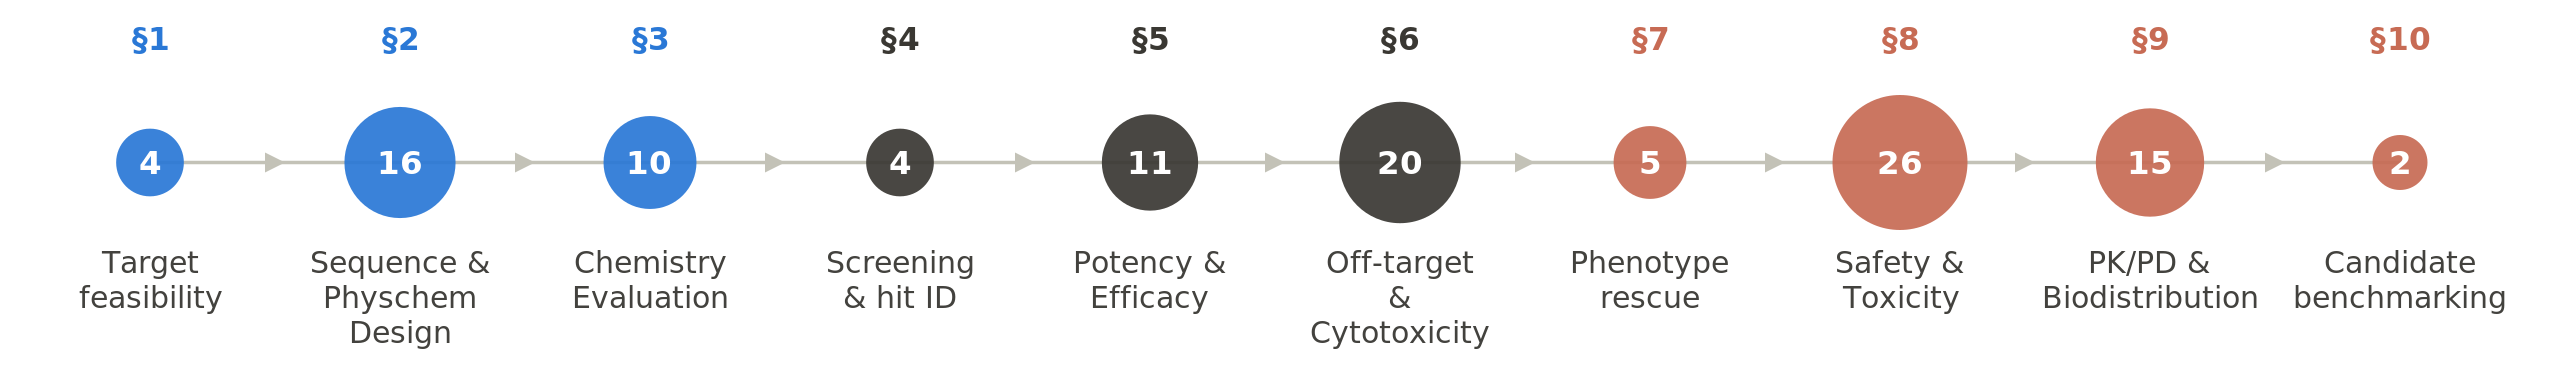
\includegraphics[width=\linewidth]{figures/chart-taxonomy.png}
\end{subfigure}
\par}
\vspace{1.4em}
{\raggedright
  \begin{subfigure}[t]{0.47\textwidth}
  \centering
  \caption{Tasks and decision types}
  \label{fig:chart-tasktype}
  \vspace{2pt}
  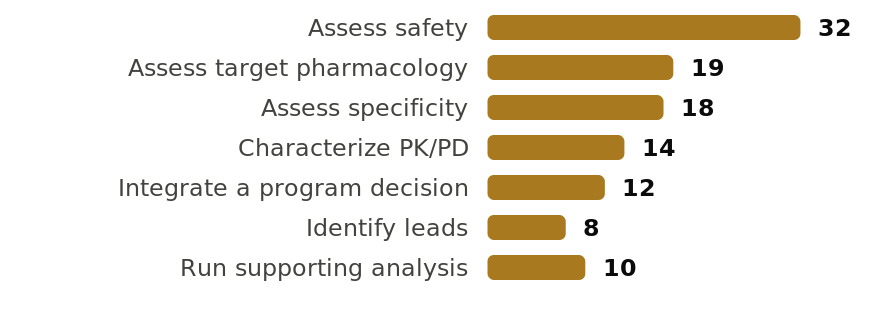
\includegraphics[width=\linewidth]{figures/chart-tasktype.png}
\end{subfigure}\hspace{1em}
  \begin{subfigure}[t]{0.47\textwidth}
  \centering
  \caption{Assay and evidence types}
  \label{fig:chart-assaytype}
  \vspace{2pt}
  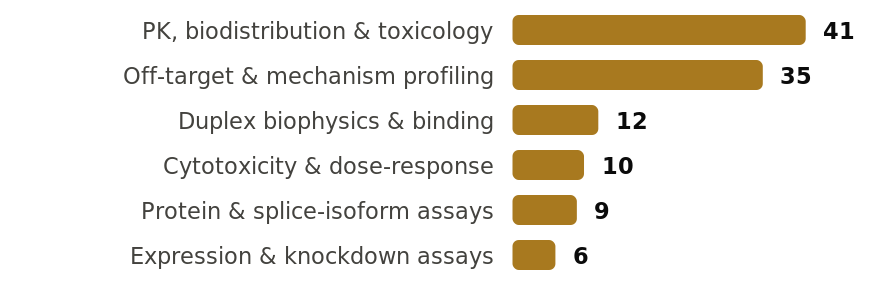
\includegraphics[width=\linewidth]{figures/chart-assaytype.png}
\end{subfigure}
\par}
\vspace{1.6em}
  \begin{subfigure}[t]{0.47\textwidth}
  \centering
  \caption{Disease indication}
  \label{fig:chart-disease}
  \vspace{2pt}
  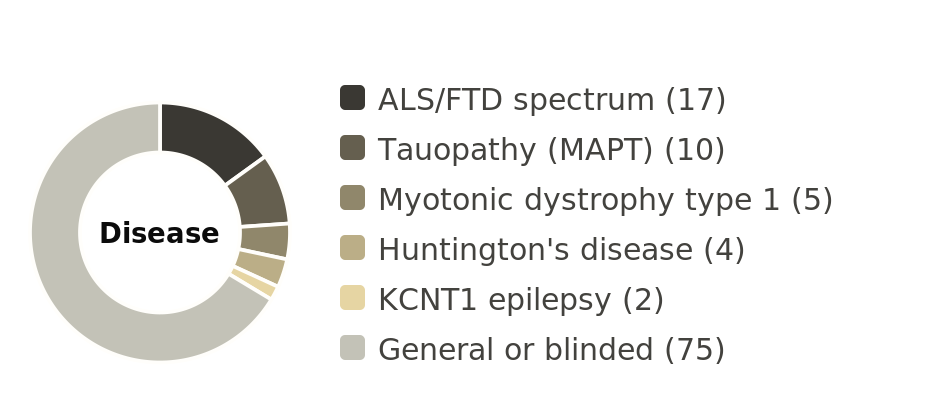
\includegraphics[width=\linewidth]{figures/chart-disease.png}
\end{subfigure}\hfill
  \begin{subfigure}[t]{0.47\textwidth}
  \centering
  \caption{Target gene}
  \label{fig:chart-genetarget}
  \vspace{2pt}
  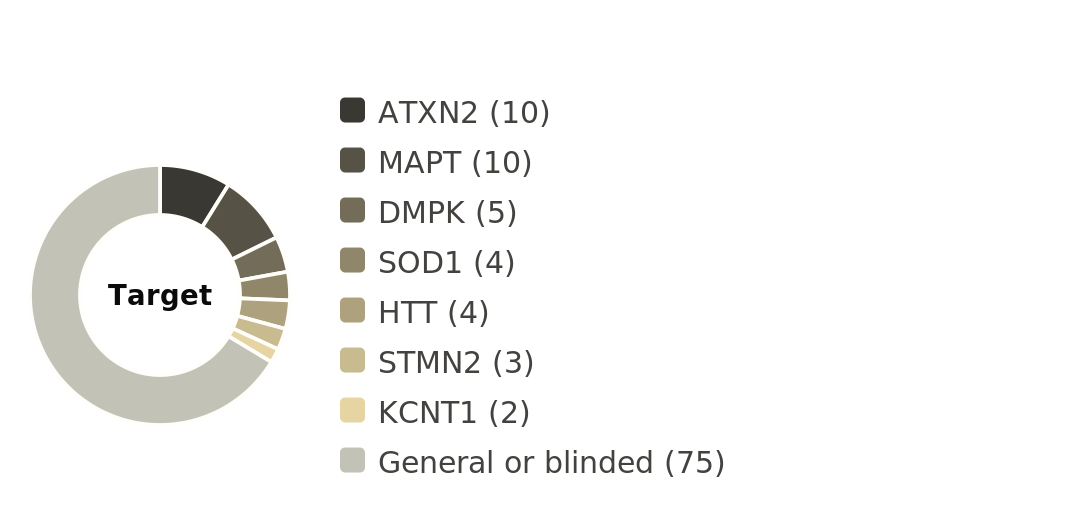
\includegraphics[width=\linewidth]{figures/chart-genetarget.png}
\end{subfigure}
\vspace{1.6em}
  \hfill\begin{subfigure}[t]{0.47\textwidth}
  \centering
  \caption{Tissue or cell type}
  \label{fig:chart-tissue}
  \vspace{2pt}
  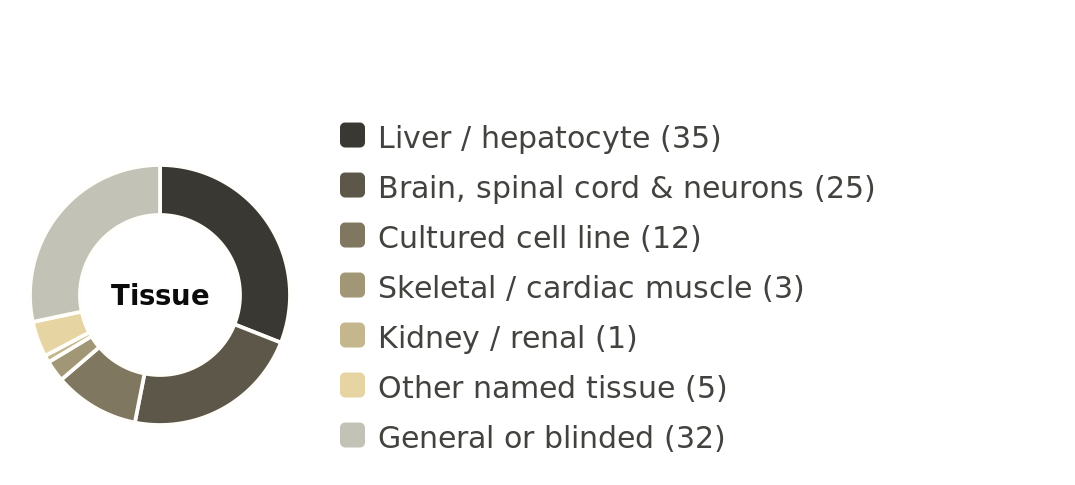
\includegraphics[width=\linewidth]{figures/chart-tissue.png}
\end{subfigure}\hfill\mbox{}
\vspace{0.6em}
\caption{\textit{Benchmark anatomy.} \quad \textbf{A,} 10-stage taxonomy of evaluations spanning discovery-to-development candidate (\S1--\S10); circle area is proportional to evaluation count. \textbf{B,} Second classification based on the type of tasks and decisions, independent of pipeline stage. \textbf{C,} Third classification based on principal assay or evidence type the underlying dataset draws from. \textbf{D,} Statistic on diseases and therapeutic indications analyzed. \textbf{E,} Statistic on gene targets included. \textbf{F,} Statistic on tissue or cell type each evaluation's dataset was generated in.}
\label{fig:fig1}
\end{figure}
\clearpage
\section{Benchmark Anatomy}
TxBench-Oligonucleotide Discovery organizes the evaluations along a 10-stage taxonomy spanning three tiers of the discovery-to-development candidate arc: target feasibility and library design (\S1--\S3), in vitro pharmacology and safety (\S4--\S6), and translational readiness (\S7--\S10) (Figure 1A). Coverage is deliberately non-uniform and focuses on stages with key data-driven program decisions. Sequence and physicochemical design (\S2), chemistry evaluation (\S3), and off-target profiling and cytotoxicity (\S6) are all well represented in the earlier and middle tiers. Coverage skews further downstream still: preclinical safety and toxicology (\S8) and in vivo PK/PD and biodistribution (\S9) together account for 41 of 113 evaluations while candidate benchmarking (\S10) has two evaluations.

A second decision-structure classification tags each evaluation by the scientific operation or judgment its passing answer requires, rather than its position in the discovery pipeline (Figure 1B). Safety assessment (32 evaluations) is the largest category, followed by target pharmacology (19), specificity assessment (18), PK/PD characterization (14); program-level integration (12), lead identification (8), and a supporting-analysis category (10) round out the remaining evaluations. While the pipeline tracks when key decision must be made, decision structure tracks what kind of judgment it demands.

A third view classifies each evaluation by the principal assay or evidence family its underlying dataset draws from (Figure 1C). PK, biodistribution, and toxicology data is the largest single family (41 of 113), closely trailed by off-target and mechanism-of-action profiling (35); together the two account for two-thirds of the set, reflecting the benchmark's emphasis on safety and exposure judgment over primary potency screening. Duplex biophysics and binding assays (12), cytotoxicity and dose-response panels (10), protein and splice-isoform readouts (9), and expression/knockdown assays (6) make up the balance.

The included indications, targets, and tissues (Figure 1D--F) cluster around a set of programs that are well known reference points in the oligonucleotide field rather than a broad therapeutic-area survey. ALS/FTD-spectrum disease and MAPT-driven tauopathy are the leading indications (Figure 1D), with myotonic dystrophy type 1, Huntington's disease, and KCNT1 epilepsy also represented; the corresponding gene targets, ATXN2, MAPT, DMPK, SOD1, HTT, STMN2, and KCNT1 (Figure 1E), are among the most extensively characterized targets in CNS and neuromuscular ASO/siRNA development, with public chemistry, off-target, and safety datasets mature enough to support deterministic grading. Tissue of origin (Figure 1F) follows the same logic.
\section{Construction Lenses and Failure-Mode Design}
\textbf{Two complementary lens families behind evaluation ideas.} A lens is a structured idea-generation heuristic used during construction to surface candidate evaluation ideas, either by mining a source paper directly or by targeting domain-specific judgment calls. TxBench-Oligonucleotide Discovery draws on two such families during construction (Figure 2A): nine general lenses (decision-mining, figure-recreation, surprises-mining, cross-source-mining, certified-references-match, skill-mining, literature-sweep, interview-questions, and trap-alignment) positioned against a source paper's Methods, figures, and Results directly, and a three-lens oligo-specific pack for modality specific problems (Key program decisions and Technical judgement, Drug development pitfalls and Optimization, ASO/siRNA quiddity).

\clearpage
\begin{figure}[p]
\centering
  \begin{subfigure}[t]{0.92\textwidth}
  \centering
  \caption{Idea generation lens library}
  \label{fig:chart-lens-pipeline}
  \vspace{2pt}
  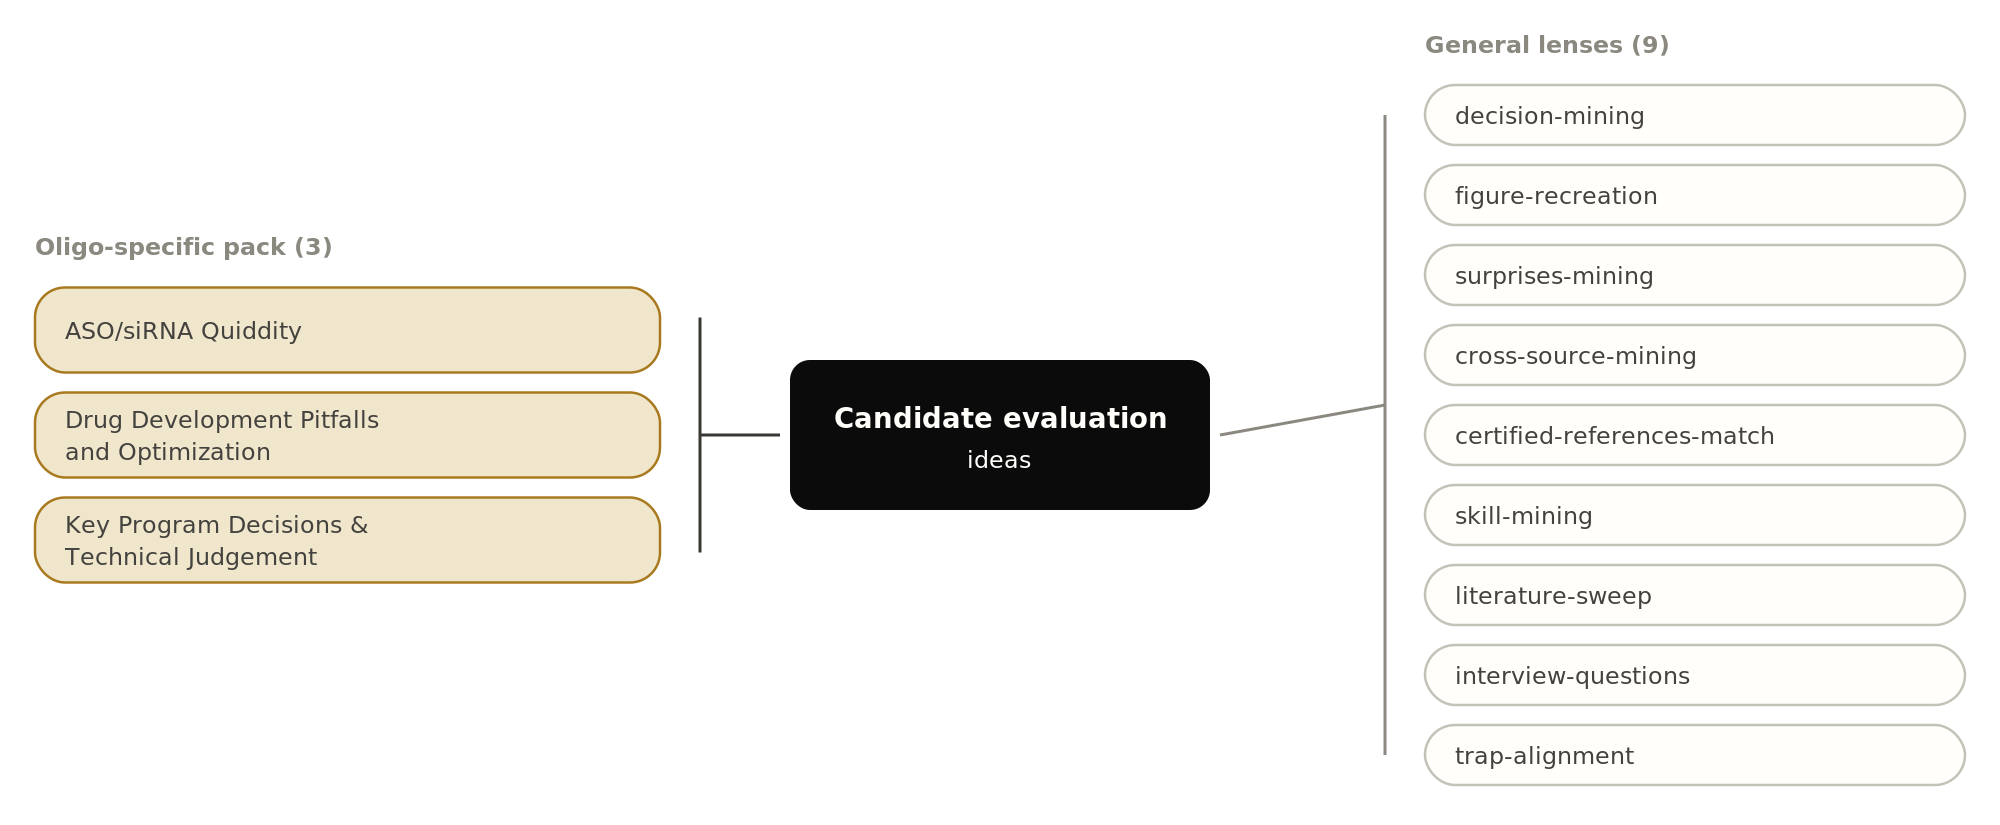
\includegraphics[width=\linewidth]{figures/chart-lens-pipeline.png}
\end{subfigure}
\vspace{0.6em}
  \begin{subfigure}[t]{0.40\textwidth}
  \centering
  \caption{Lens alignment summary}
  \label{fig:chart-lens}
  \vspace{2pt}
  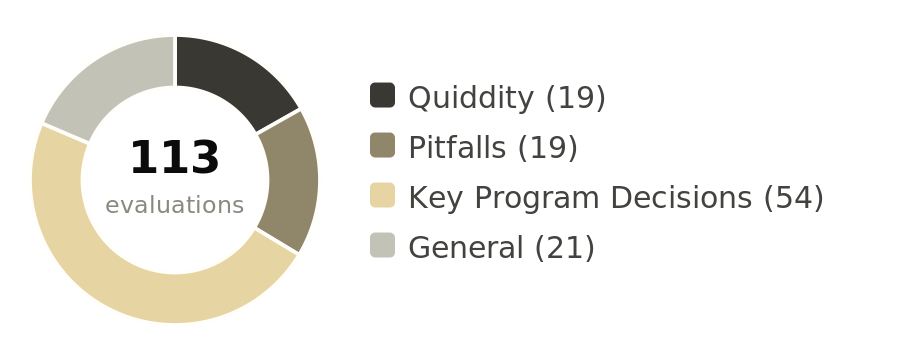
\includegraphics[width=\linewidth]{figures/chart-lens.png}
\end{subfigure}\hfill
  \begin{subfigure}[t]{0.50\textwidth}
  \centering
  \caption{Key Program Decisions \& Technical Judgement lens}
  \label{fig:chart-kjd}
  \vspace{2pt}
  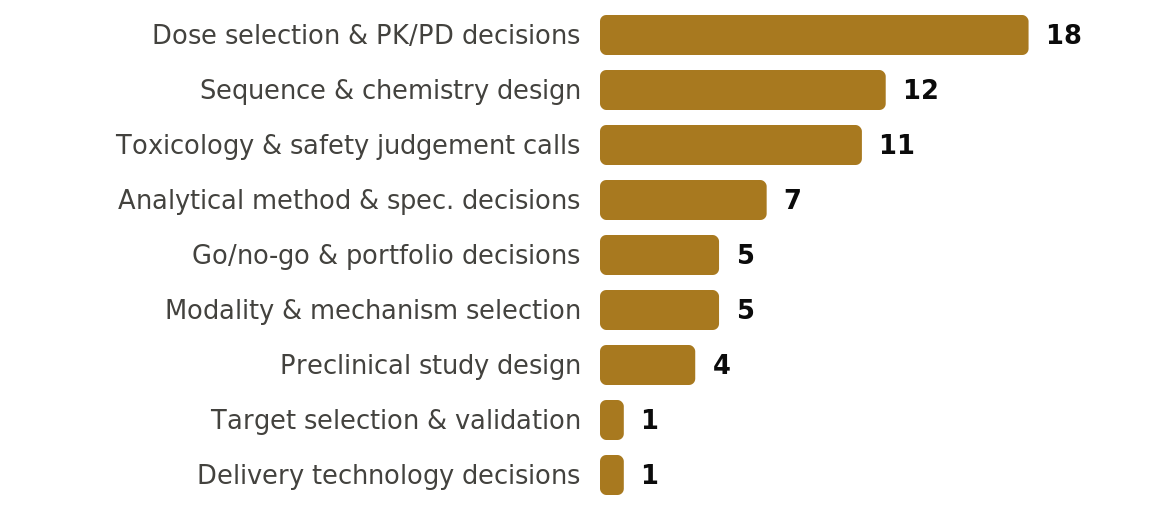
\includegraphics[width=\linewidth]{figures/chart-kjd.png}
\end{subfigure}
\vspace{0.6em}
  \begin{subfigure}[t]{0.47\textwidth}
  \centering
  \caption{Grader type usage}
  \label{fig:chart-gradertype}
  \vspace{2pt}
  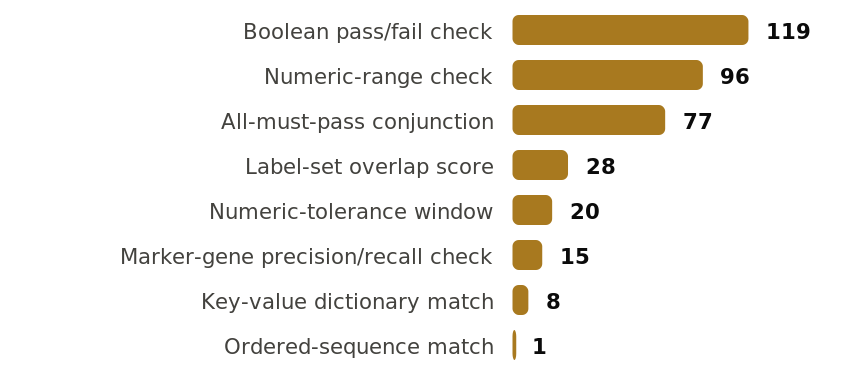
\includegraphics[width=\linewidth]{figures/chart-gradertype.png}
\end{subfigure}\hfill
  \begin{subfigure}[t]{0.47\textwidth}
  \centering
  \caption{Per-eval failure mode tags}
  \label{fig:chart-failuremode}
  \vspace{2pt}
  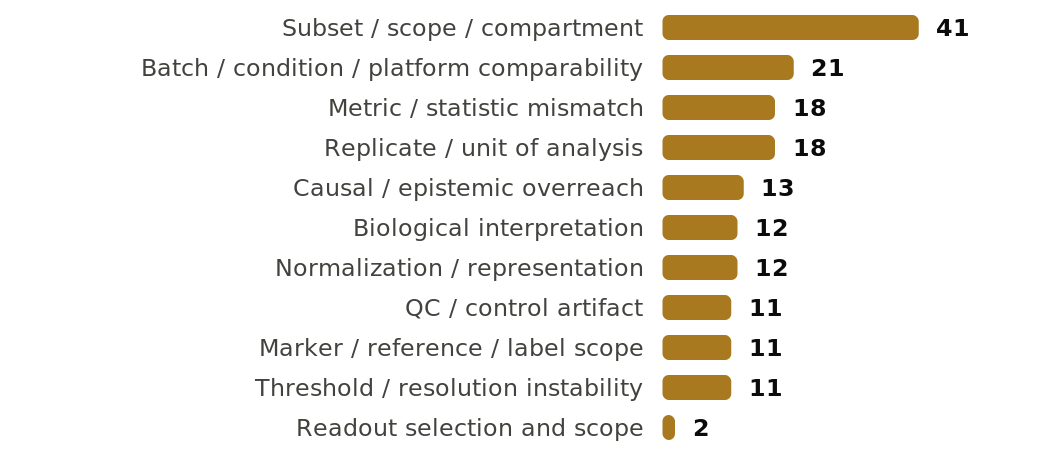
\includegraphics[width=\linewidth]{figures/chart-failuremode.png}
\end{subfigure}
\vspace{0.6em}
\caption{\textit{Construction lenses and failure-mode design.} \quad \textbf{A,} Idea-generation lens library: nine general lenses plus a three-lens oligo-specific pack for modality specific problem; both part the same logic construction pipeline. \textbf{B,} Evaluation counts across each modality-specific lens and general. \textbf{C,} Representation of Key program decisions and Technical judgment lens subcategories; \textbf{D,} Grader-type usage in the 113 evaluations; \textbf{E,} Per-evaluation failure-mode tags, populated on 55 of 113 evaluations (170 tag instances).}
\label{fig:fig2}
\end{figure}
\clearpage

The three oligo-specific lenses are represented with 54 evaluations for Key program decisions and Technical judgment and 19 each for Drug development pitfalls and Optimization and ASO/siRNA quiddity (Figure 2B), remaining 21 evaluations were aligned with the general lenses. Because the three named lenses' alignment is not mutually exclusive (a single evaluation can align with more than one), the general slice is an upper bound on general-only coverage, not an exact count.

The Key program decisions lens (twelve categories of real development judgment calls, from target selection through regulatory strategy) accounts for the largest matched share of the three oligo-specific lenses. Its evaluations break down across nine of the lens's twelve categories (Figure 2C): dose selection and PK/PD decisions is the largest, followed by sequence and chemistry design and toxicology and safety judgement calls.

Every evaluation is graded by a deterministic, multi-part grader rather than a single tolerance check (Figure 2D), assembled from leaf checks: atomic, single-criterion checks, as distinct from a composition wrapper that combines multiple checks into one verdict. Boolean pass/fail gates (119 instances) and numeric-range bands (96) are the two most common leaf types, typically composed under an all-must-pass conjunction (77 instances), which requires a correct answer on each component for an agent to pass, mirroring real-life decision outcomes in drug discovery. Label-set overlap scores, symmetric numeric-tolerance windows, marker-gene precision/recall floors, per-key dictionary matches, and a single ordered-sequence match check round out the remaining grader vocabulary.

\textbf{Failure modes are tagged directly at construction.} A per-evaluation failure-mode taxonomy tags each evaluation with its trap: a specific scientific failure mode a grader is deliberately built to catch, tagged at construction time (Figure 2E). This field is populated on 55 of 113 evaluations (170 tag instances) and is dominated by subset/scope/compartment errors: picking the wrong biological subset, comparator, or baseline rather than making an arithmetic mistake. Batch/condition/platform comparability, metric/statistic mismatch, and replicate/unit-of-analysis errors follow; causal/epistemic overreach, biological interpretation, and normalization/representation errors contribute roughly equal shares, with QC/control-artifact, marker/reference/label-scope, and threshold/resolution-instability errors filling out the remainder. This distribution closely mirrors the failure taxonomies reported for TxBench-Antibody (scope/denominator/estimand errors: 34.7\% of evaluable failures) and TxBench-PP (method and calibration errors: 71\% of reviewed failures), suggesting this may be a cross-modality attractor for agent failure in decision-centered biology benchmarks generally.
\begin{quote}
\noindent\rule{\linewidth}{0.4pt}\\[2pt]
\textbf{Design note.} A grader is only useful if failure is well-specified: the philosopher of science Karl Popper's requirement that a test admit a decisive way to fail (Popper 1959), which is what the boolean pass/fail and numeric-range checks are built to do. But when an evaluation fails, the Duhem--Quine thesis applies (no hypothesis can be tested in isolation from the auxiliary assumptions bundled with it; Duhem 1954, Quine 1951): the failure can be attributed to the target decision or to an auxiliary interpretive choice bundled with it (scope, comparator, baseline), which is why the failure-mode taxonomy (Figure 2E) is dominated by scope/comparator errors rather than raw computation.\\[2pt]\rule{\linewidth}{0.4pt}
\end{quote}
\section{Results}
\textbf{No configuration exceeds 56\% of endpoint attempts.} The full campaign covers 113 evaluations across 21 model-harness configurations (12 models $\times$ 4 execution harnesses: Pi, Claude Code, OpenAI Codex, Grok Build), for 7,098 valid grading runs, with agents working in a sandboxed environment with no internet access. Pass rate is defined per evaluation as correct results over valid grading runs, then averaged across evaluations per configuration; error bars are 95\% Student-t intervals over those per-evaluation means, matching the convention used in TxBench-PP and TxBench-Antibody. The strongest configuration, GPT-6 Astra on OpenAI Codex, passed 55.5\% of endpoint attempts (95\% CI 47.2--63.7); pooled across every configuration, agents passed 38.5\% of valid grading runs (2,730/7,098) (Figure 3A).

Repeatability across the three attempts per evaluation (Figure 3B) shows the same pattern reported for TxBench-PP and TxBench-Antibody: a configuration that fails once usually fails all three times rather than splitting evenly, and the strongest configurations still fail all three attempts on roughly a third of evaluations (34--36\%).

\begin{figure}[!htbp]
\centering
  \begin{subfigure}[t]{0.47\textwidth}
  \centering
  \caption{Model--harness pass rate}
  \label{fig:chart-fig3-passrate}
  \vspace{2pt}
  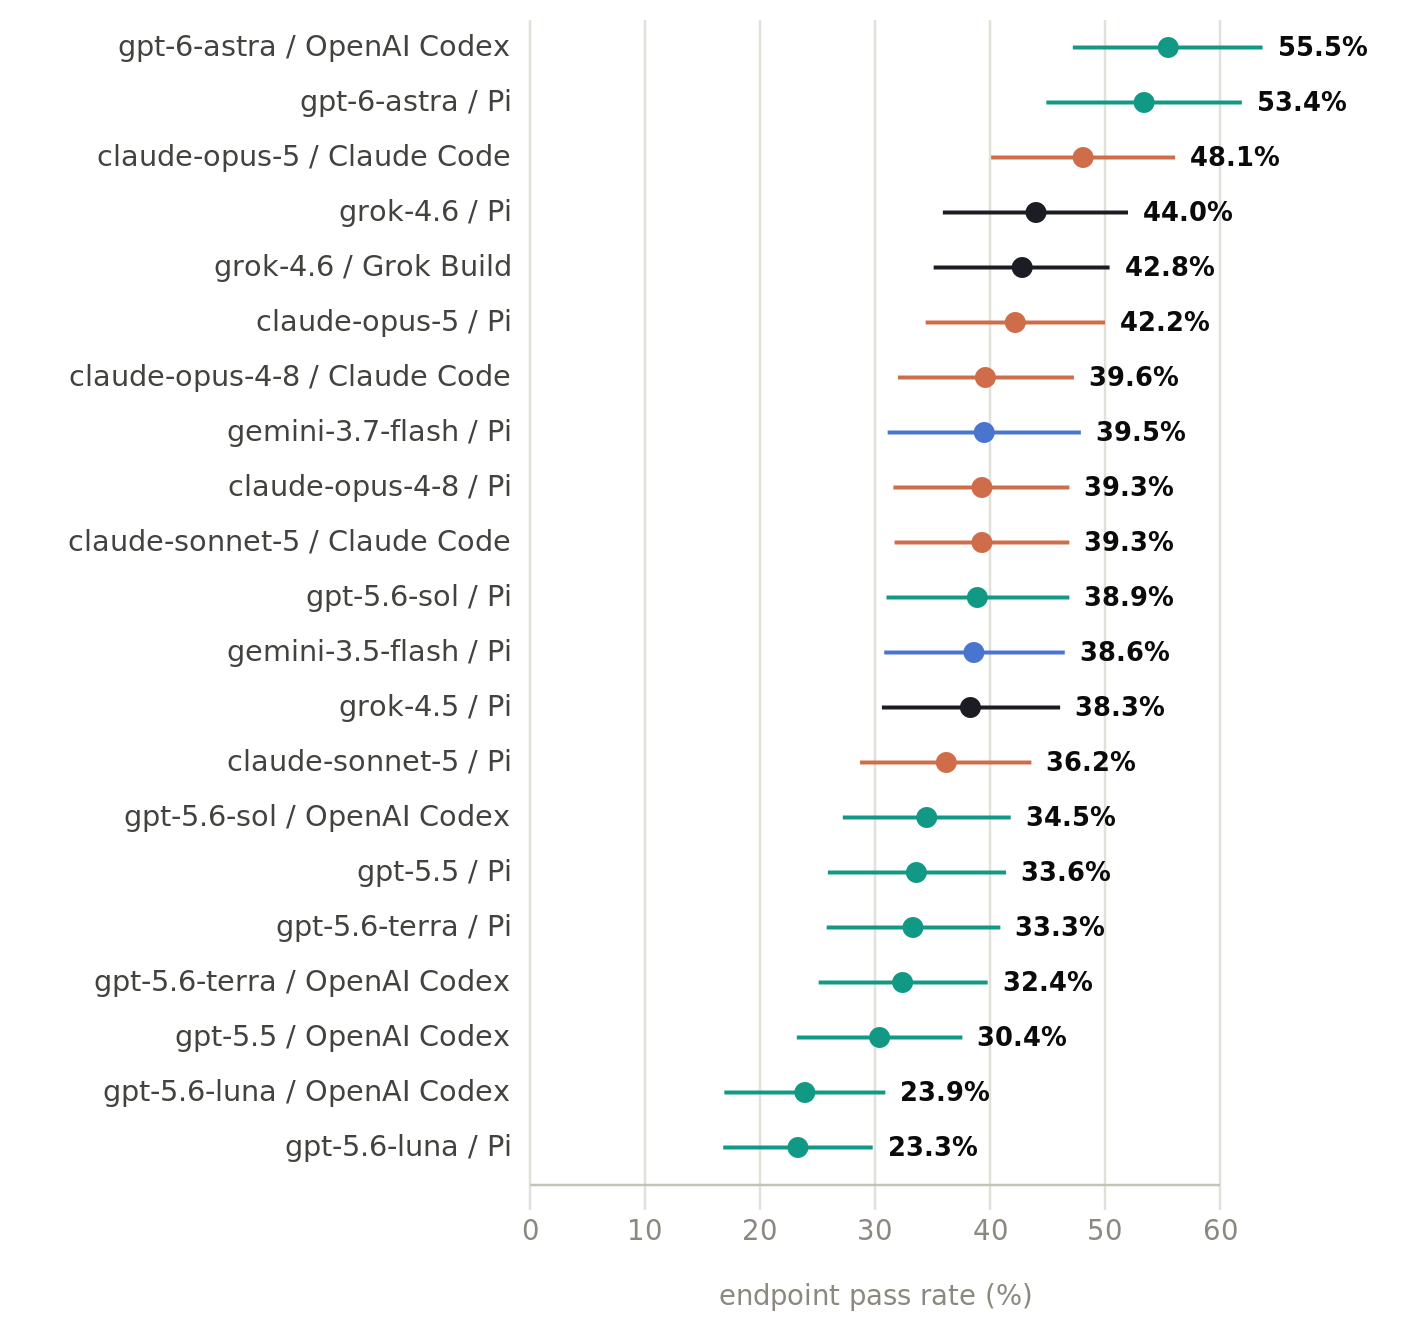
\includegraphics[width=\linewidth]{figures/chart-fig3-passrate.png}
\end{subfigure}\hfill
  \begin{subfigure}[t]{0.47\textwidth}
  \centering
  \caption{Repeatability across three attempts}
  \label{fig:chart-fig3-repeat}
  \vspace{2pt}
  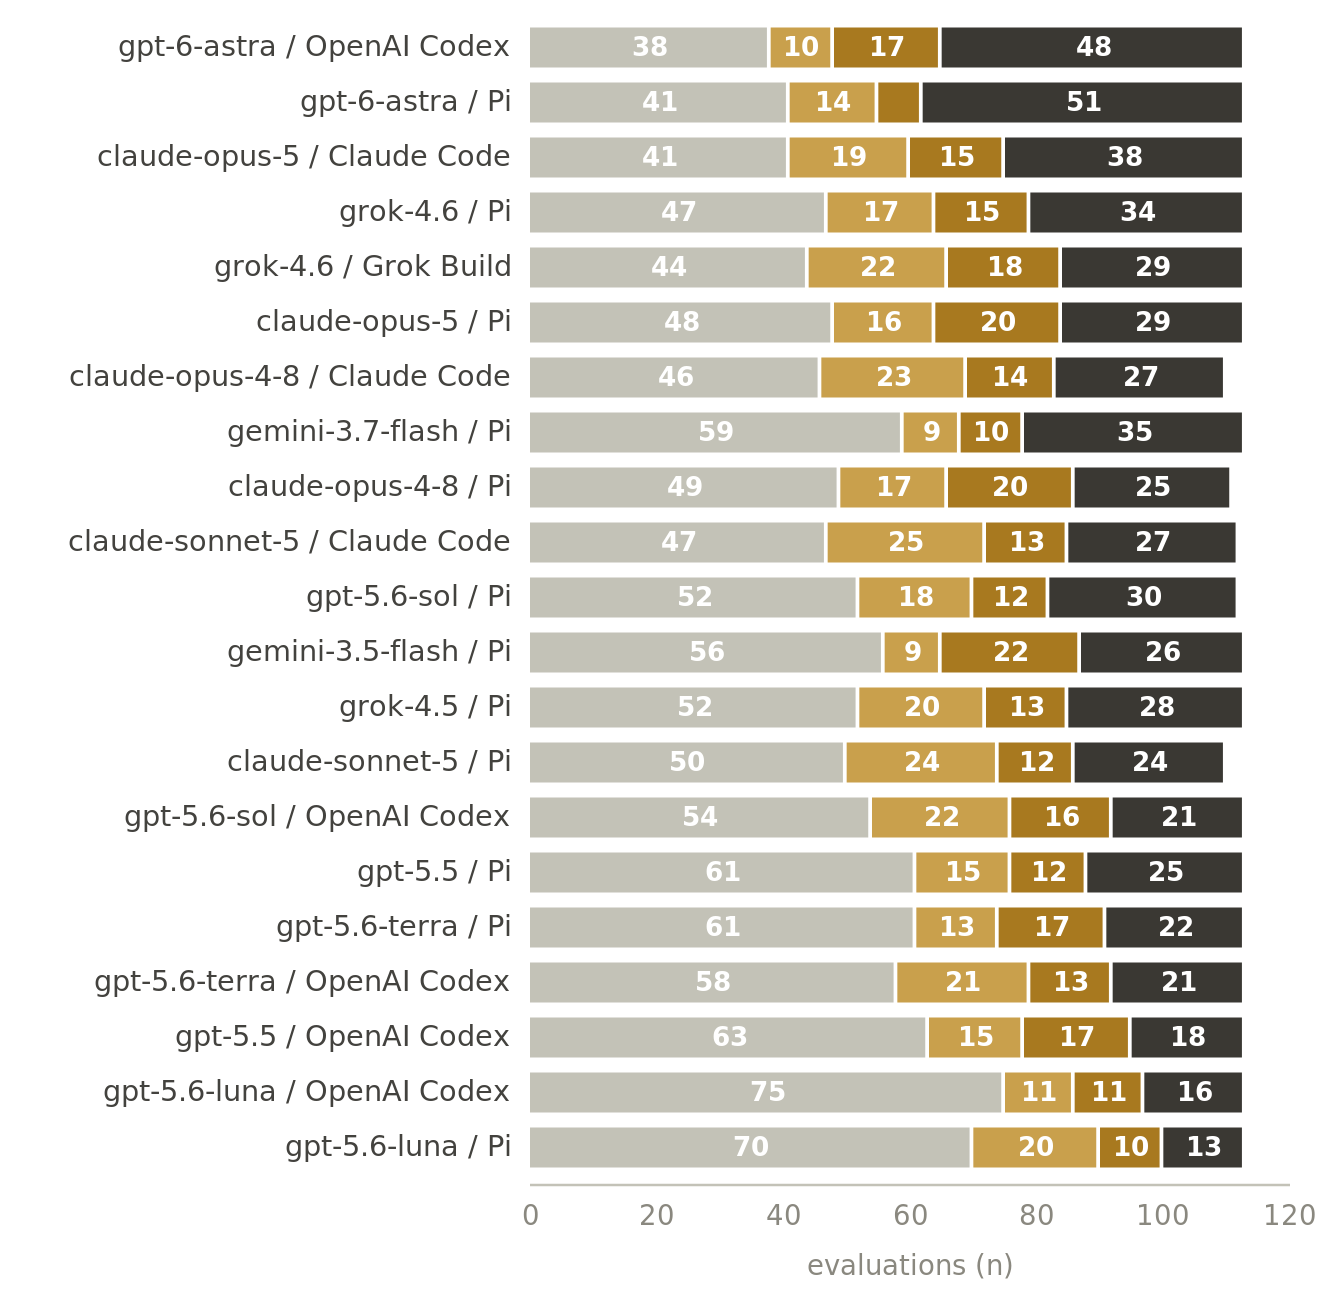
\includegraphics[width=\linewidth]{figures/chart-fig3-repeat.png}
\end{subfigure}
\vspace{0.6em}
\caption{\textit{Endpoint pass rate and repeatability.} \quad \textbf{A,} Model--harness pass rate across all 21 configurations (95\% CI over per-evaluation means; n=113 evaluations/configuration, fewer for four configurations with partial platform failures, see execution-reliability discussion below). \textbf{B,} Repeatability across the three attempts per evaluation; bars sum to the evaluations with a complete triplicate.}
\label{fig:fig3}
\end{figure}

\textbf{Harness choice shows a consistent home-field pattern for Claude, but not for GPT.} Matched Pi-vs-alternate-harness comparisons (Figure 4) are available for nine of the twelve models (the three Gemini configurations and Grok 4.5 were only run on Pi). All three Claude checkpoints score higher on Claude Code than on Pi (Opus 5: 42.2\% vs. 48.1\%, $\Delta$=$-$5.9; Sonnet 5: 36.2\% vs. 39.3\%, $\Delta$=$-$3.1; Opus 4.8: 39.3\% vs. 39.6\%, $\Delta$=$-$0.4), a uniform advantage for the family's own harness, though the size of that advantage varies considerably. GPT shows no equivalent pattern: GPT-6 Astra and GPT-5.6-luna score marginally higher on OpenAI Codex ($\Delta$=$-$2.1 and $-$0.6), while GPT-5.6-sol, GPT-5.5, and GPT-5.6-terra score higher on Pi instead ($\Delta$=+4.4, +3.2, +0.9); three of five GPT configurations favor the non-native harness. The one available Grok comparison, Grok 4.6, also favors Pi over its own Grok Build harness ($\Delta$=+1.2). Across all nine comparisons the mean absolute shift is 2.4 points (median 2.1), bounded by Claude Opus 5 ($-$5.9) and GPT-5.6-sol (+4.4) at the extremes; each configuration's own 95\% CI is wide enough to overlap the other harness's point estimate in every one of the nine pairs, so none of these differences should be read as a settled reversal, only as evidence that harness is a real, if second-order, source of variance in reported pass rate.

\begin{figure}[!htbp]
\centering
{\raggedright
  \begin{subfigure}[t]{0.92\textwidth}
  \centering
  \caption{Score difference across harnesses}
  \label{fig:chart-full-harnessdelta}
  \vspace{2pt}
  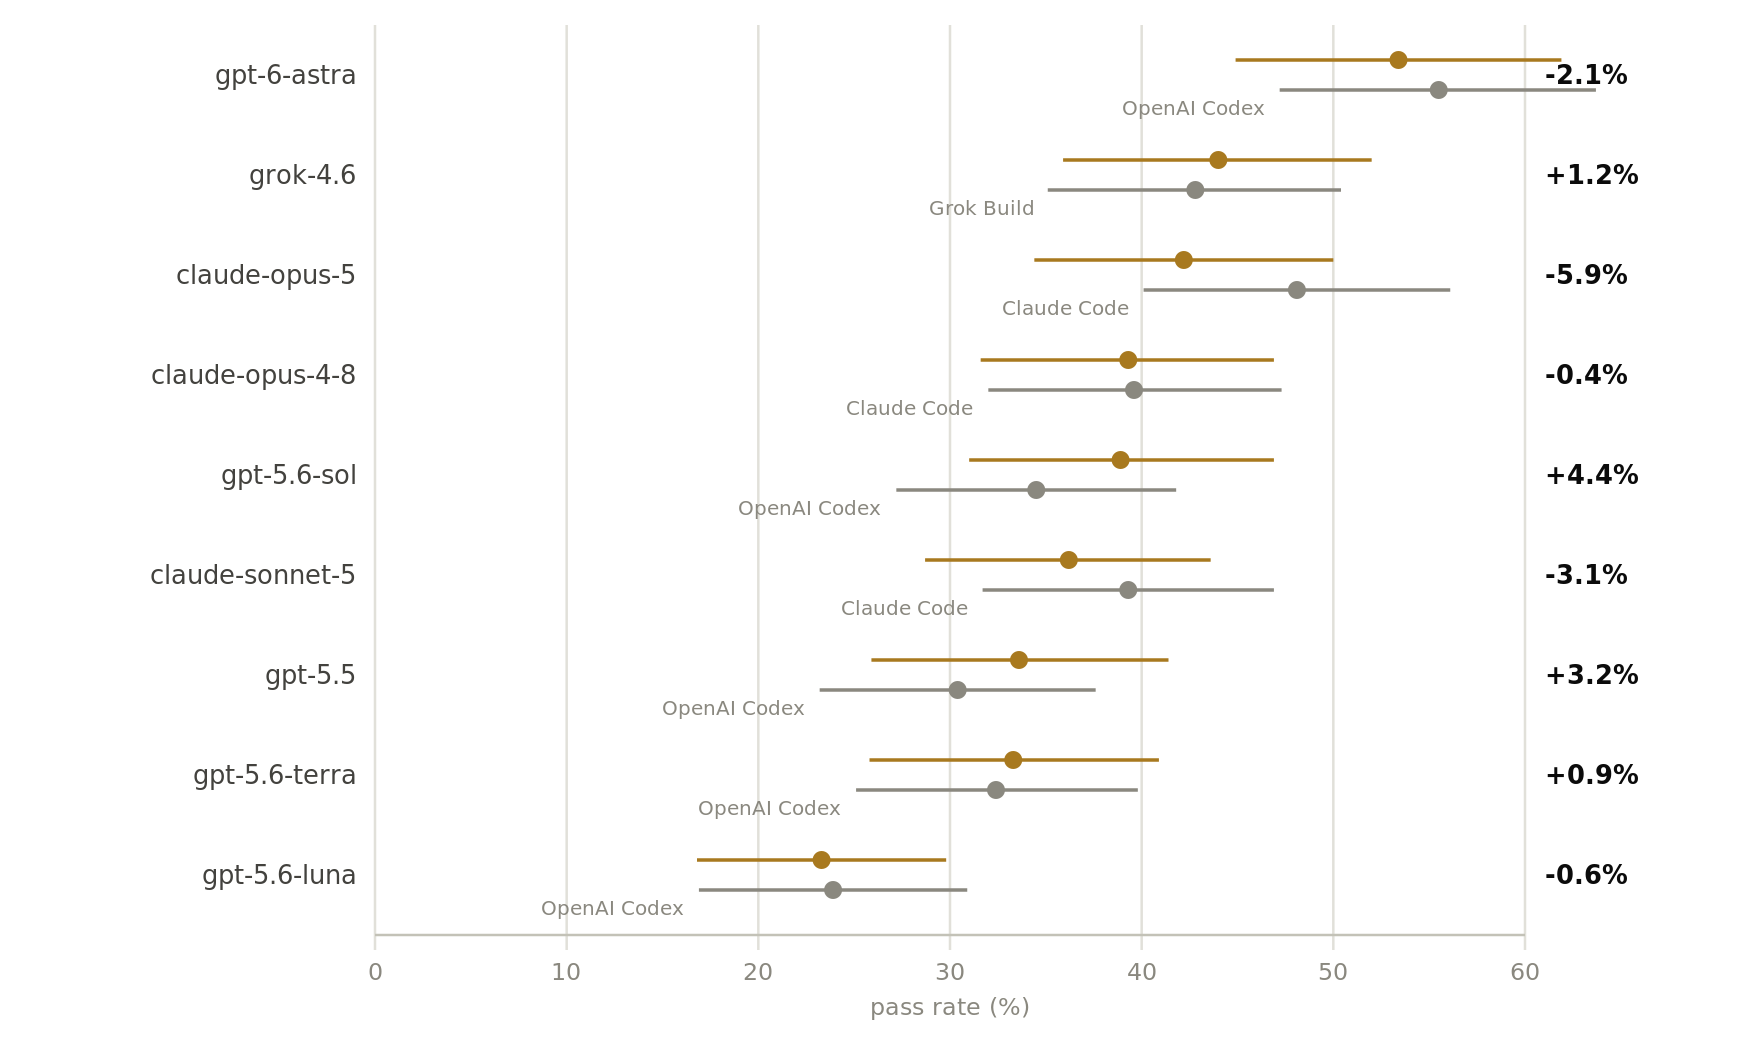
\includegraphics[width=\linewidth]{figures/chart-full-harnessdelta.png}
\end{subfigure}
\par}
\vspace{0.6em}
\caption{\textit{Score difference across harnesses.} \quad Matched Pi-versus-alternate-harness score differences within the same model (95\% CI whiskers).}
\label{fig:fig4}
\end{figure}
\FloatBarrier
\textbf{Individual models diverge even when aggregate pass rates look similar.} Reducing each evaluation to a per-model pass/fail verdict and comparing all 66 pairs across the 12 models surfaces real structure with Cohen's kappa (chance-corrected agreement on the same binarized verdicts) ranging from $-$0.01 to 0.56, mean 0.24. This represents slight-to-moderate agreement, though not a clean per-family partition visualized in a 2-D similarity map (Figure 5). GPT-6 Astra sits apart from every other model, at the greatest mean distance from the other eleven models (mean kappa 0.16), the lowest of any model. Claude Sonnet 5 is the one model whose closest pairing crosses family lines: it clusters with Gemini 3.5 Flash (kappa 0.32) rather than with Claude Opus 4.8 (kappa 0.27) or Opus 5 (kappa 0.23), which instead pair more closely with Gemini 3.7 Flash and the grok-4.5/4.6 pair. 

The full pairwise agreement matrix (Figure 6A) gives the exact per-pair values behind that picture. Evaluation-level head-to-head comparisons for three representative pairs confirm this isn't aggregate noise: GPT-6 Astra beat Claude Opus 5 on 54 evaluations against 32 in the other direction (27 tied; Figure 6B; kappa 0.07), a similar pattern to its comparison against Grok 4.6 (50 against 33, 30 tied; Figure 6C; kappa 0.14). The comparison between Claude Opus 5 and Grok 4.6 (Figure 6D) is more evenly split (38 against 36, 39 tied; kappa 0.28).

\begin{figure}[!htbp]
\centering
  \begin{subfigure}[t]{\textwidth}
  \centering
  \caption{Cross-model agreement, 2D map}
  \label{fig:chart-sim-mds}
  \vspace{2pt}
  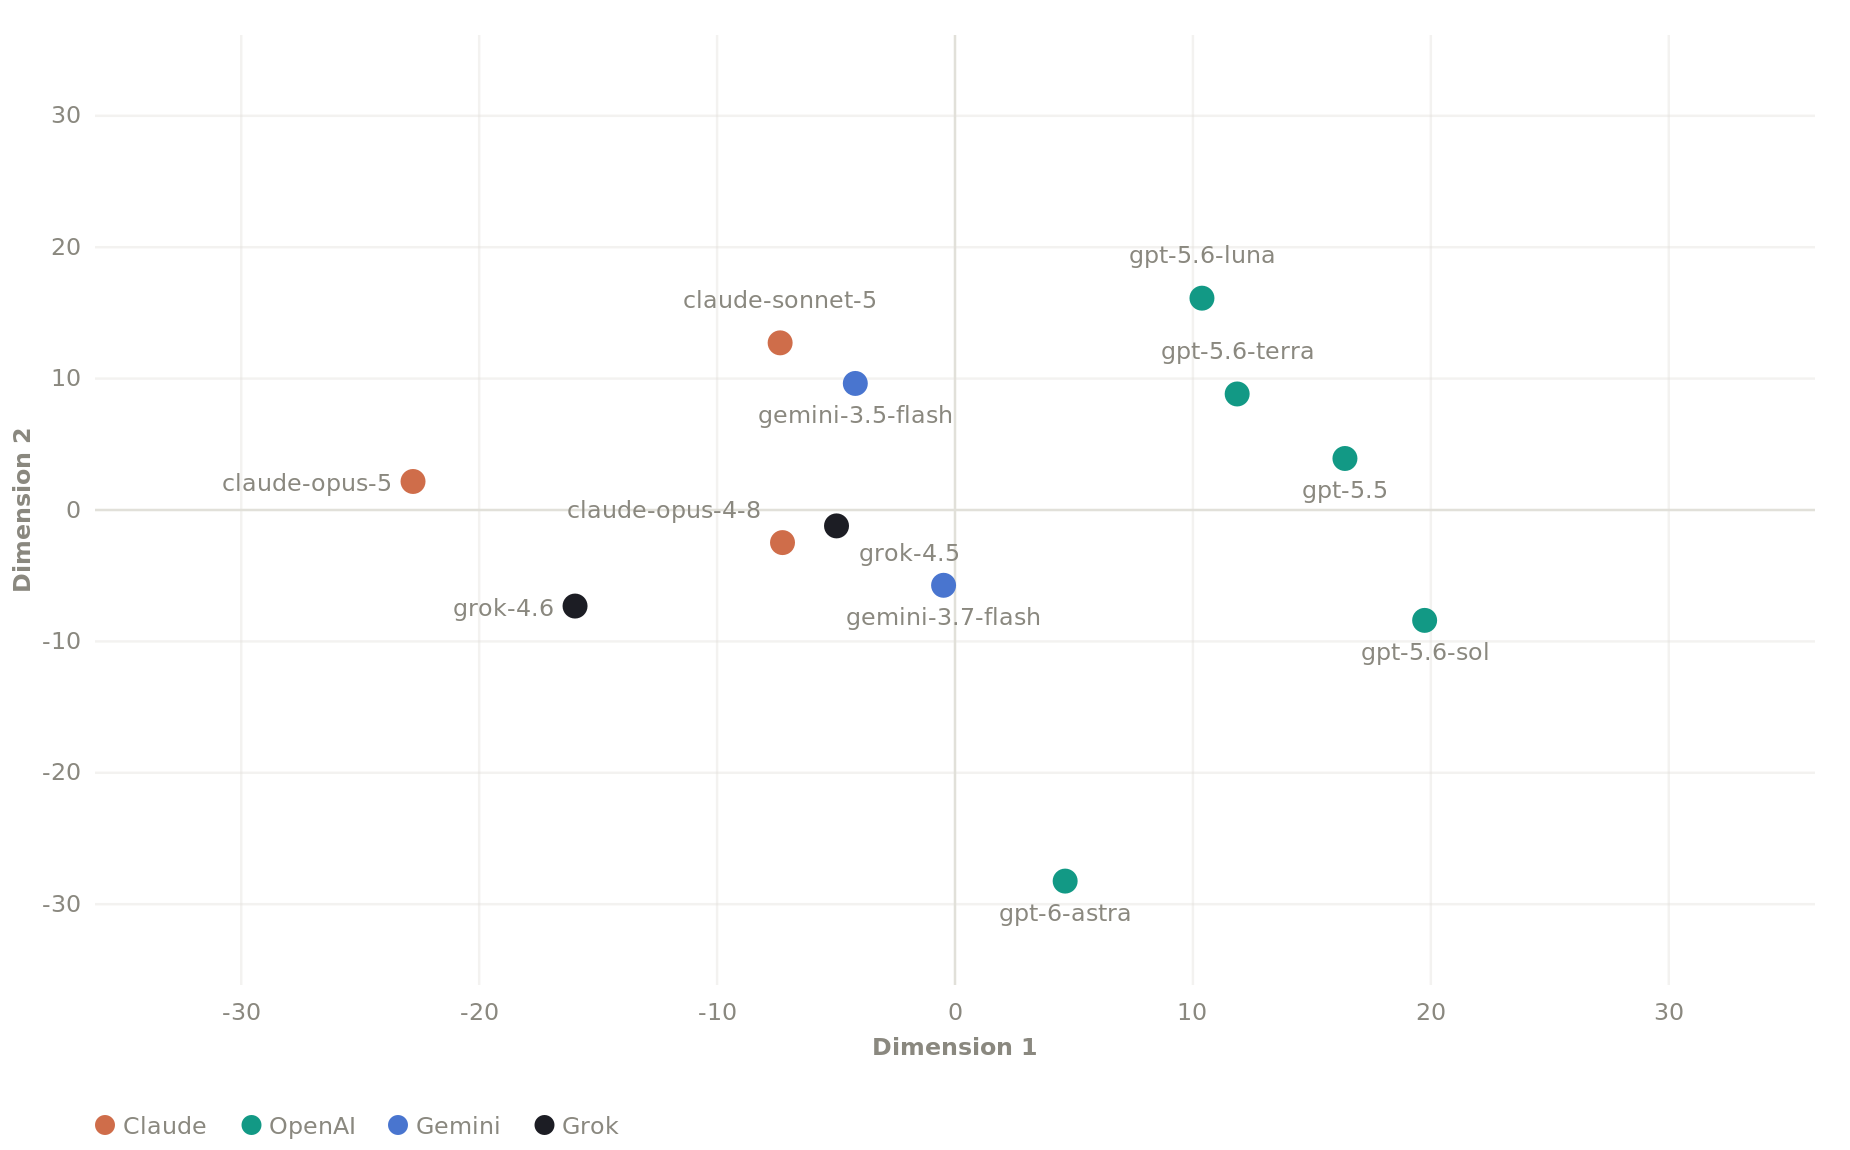
\includegraphics[width=\linewidth]{figures/chart-sim-mds.png}
\end{subfigure}
\vspace{0.6em}
\caption{\textit{Cross-model agreement, 2-D similarity map.} \quad 2-D similarity map (classical multidimensional scaling on pairwise evaluation-level agreement, treated as a distance) across all 12 models; arbitrary units, first two dimensions capture 46\% of total variance. Cohen's kappa on the same pairwise verdicts ranges $-$0.01--0.56 across the 66 pairs (mean 0.24).}
\label{fig:fig5}
\end{figure}

\begin{figure}[p]
\centering
  \begin{subfigure}[t]{0.47\textwidth}
  \centering
  \caption{Pairwise agreement matrix}
  \label{fig:chart-sim-matrix}
  \vspace{2pt}
  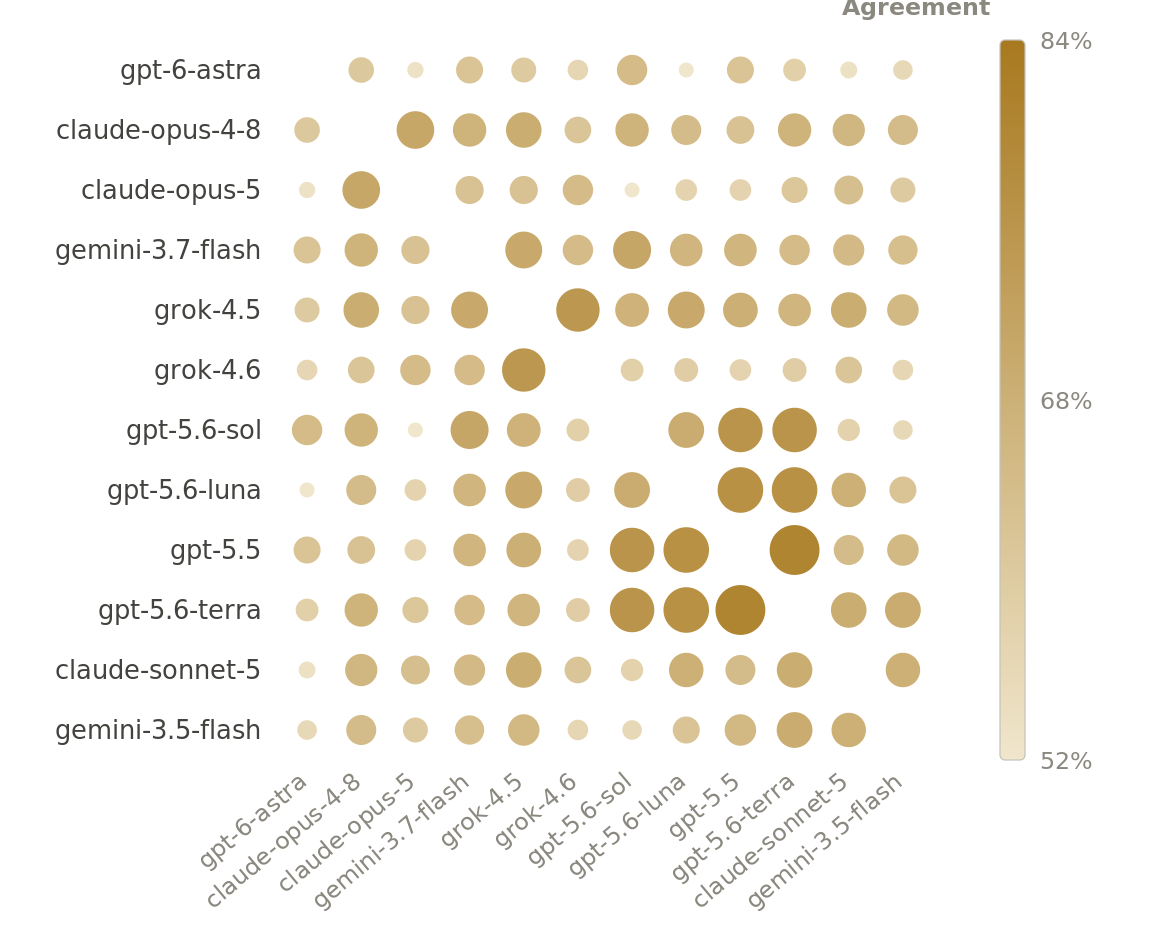
\includegraphics[width=\linewidth]{figures/chart-sim-matrix.png}
\end{subfigure}\hfill
  \begin{subfigure}[t]{0.47\textwidth}
  \centering
  \caption{GPT-6 Astra vs. Claude Opus 5}
  \label{fig:chart-h2h-1}
  \vspace{2pt}
  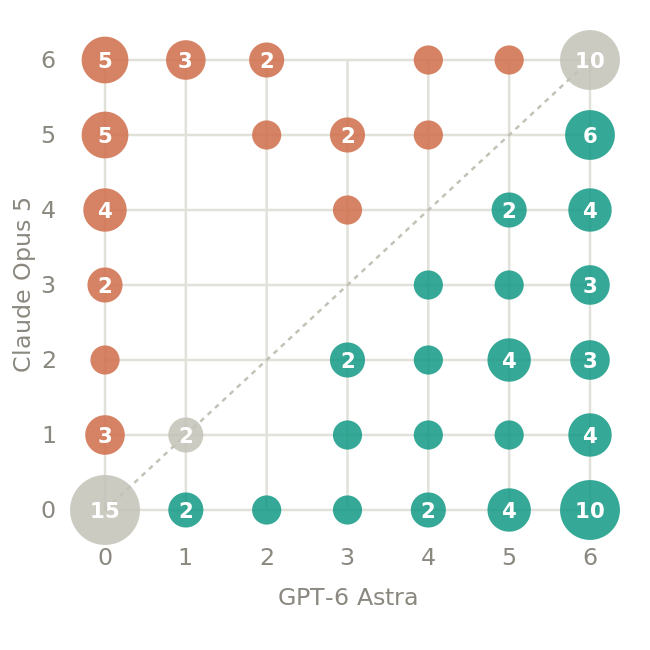
\includegraphics[width=\linewidth]{figures/chart-h2h-1.png}
\end{subfigure}
\vspace{0.6em}
  \begin{subfigure}[t]{0.47\textwidth}
  \centering
  \caption{GPT-6 Astra vs. Grok 4.6}
  \label{fig:chart-h2h-2}
  \vspace{2pt}
  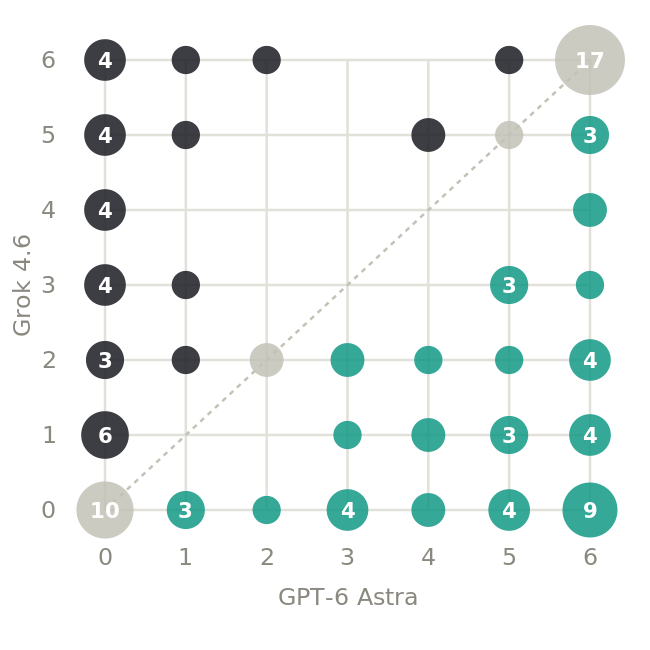
\includegraphics[width=\linewidth]{figures/chart-h2h-2.png}
\end{subfigure}\hfill
  \begin{subfigure}[t]{0.47\textwidth}
  \centering
  \caption{Claude Opus 5 vs. Grok 4.6}
  \label{fig:chart-h2h-3}
  \vspace{2pt}
  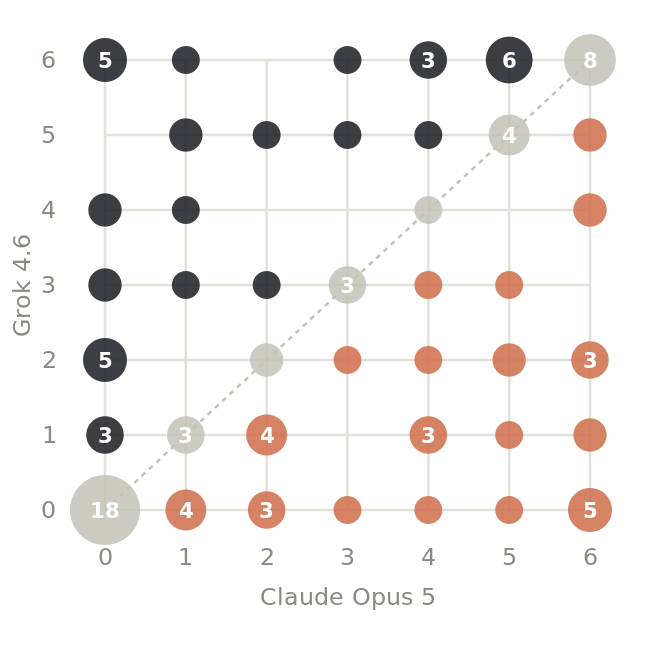
\includegraphics[width=\linewidth]{figures/chart-h2h-3.png}
\end{subfigure}
\vspace{0.6em}
\caption{\textit{Pairwise agreement matrix and evaluation-level head-to-head comparisons.} \quad \textbf{A,} Full pairwise agreement matrix (percent of evaluations where both models' pass/fail verdicts match), ordered by hierarchical clustering; diagonal omitted. \textbf{B,} GPT-6 Astra versus Claude Opus 5. \textbf{C,} GPT-6 Astra versus Grok 4.6. \textbf{D,} Claude Opus 5 versus Grok 4.6. Panels B--D pool a model's two execution harnesses (3 attempts each) into 0--6 successes per evaluation; bubble area is proportional to evaluation count, and bubble color follows the family color of whichever axis model wins that evaluation (gray marks is a tie).}
\label{fig:fig6}
\end{figure}
\clearpage
\textbf{Pass rate varies substantially across the taxonomy.} GPT-6 Astra is the strongest configuration across the three middle, more procedural pipeline stages: screening \& hit-calling (\S4, 75.0\%), potency \& efficacy (\S5, 63.6\%), and off-target \& cytotoxicity (\S6, 56.7\%); several of its clearest wins there are large-table quantitative tasks: computing dose-response potency parameters from large patent-derived knockdown tables, confirming a prospectively-ranked potency screen against a fixed confirmation-assay condition, and attributing transcriptome-wide splicing changes to an oligonucleotide's own predicted binding site rather than off-target noise; each reaches 100\% for GPT-6 Astra against 0--33\% for the other three families on the identical evaluation. Claude Opus 5 shows the opposite specialization, performing well in phenotype rescue (\S7, 73.3\% vs. 0--20\% for the rest) and other tasks that require biological judgment about a disease model's functional outcome rather than a knockdown percentage: reading Kaplan--Meier survival curves in a disease-model animal study, interpreting immunohistochemical tissue staining as a disease-phenotype endpoint, and judging whether a reported functional or clinical score constitutes real efficacy benefit; Opus passes these outright where the other three families mostly fail. No configuration is uniformly weakest at the same stage: Gemini 3.7 Flash reaches 0\% at phenotype rescue (\S7) and candidate benchmarking (\S10), the latter on an n=2 floor where a single evaluation swings the whole rate; read \S10 with the same caution already noted for Figure 1A.

\begin{figure}[!htbp]
\centering
  \begin{subfigure}[t]{0.92\textwidth}
  \centering
  \caption{Pass rate by taxonomy section}
  \label{fig:chart-full-stage}
  \vspace{2pt}
  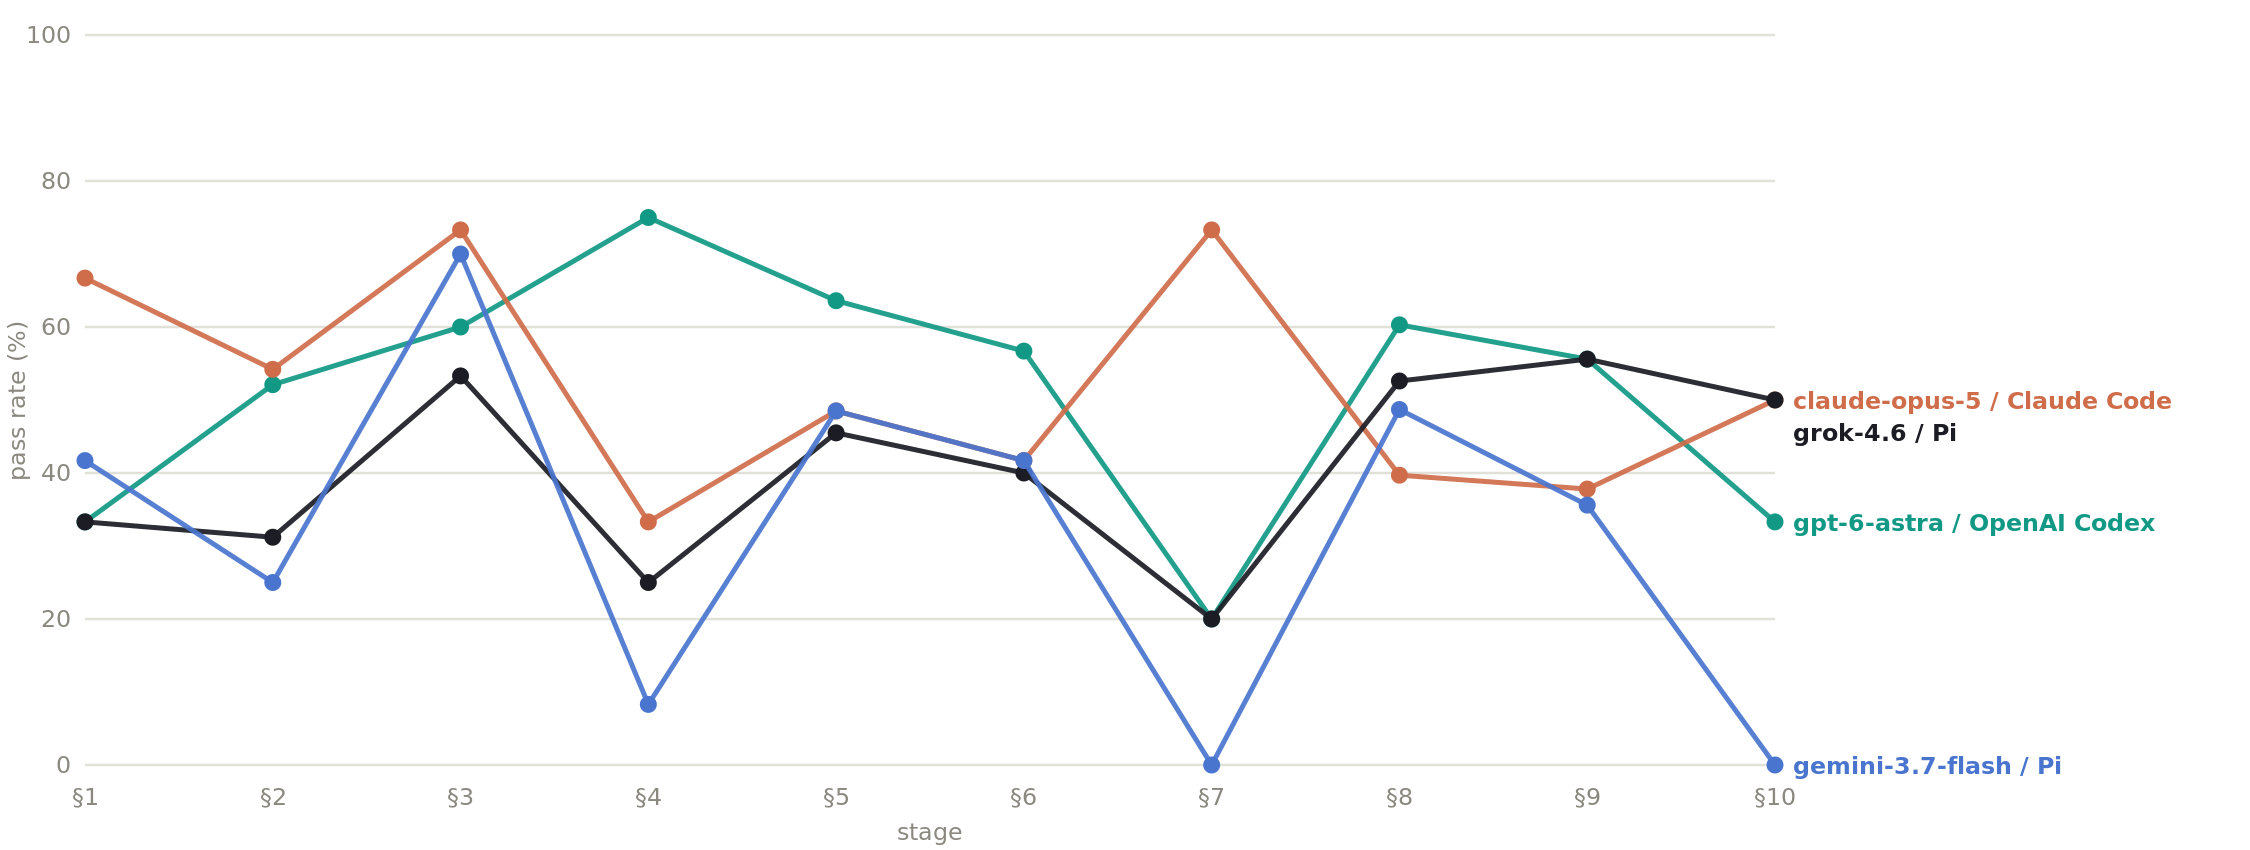
\includegraphics[width=\linewidth]{figures/chart-full-stage.png}
\end{subfigure}
\vspace{0.6em}
\caption{\textit{Pass rate by taxonomy section.} \quad Pass rate by the same \S1--\S10 discovery-stage taxonomy as Figure 1A; top configuration per family highlighted.}
\label{fig:fig7}
\end{figure}

\textbf{Experimental evidence type separates strong and weak performance sharply.} Pass rate spans a wider range across experimental problems (Figure 8): oligo sequence design (53.7\% mean), dose response (53.3\%), and organ/tissue toxicity (51.9\%) are the strongest categories, while splicing/isoform analysis (15.2\%) and RNA-seq (20.7\%) are the weakest, a wider spread than separates the strongest model overall, GPT-6 Astra (49.8\% mean), from the weakest, gpt-5.6-luna (20.4\%). The matrix's highest cell, 72\%, is reached twice, by Claude Opus 5 on dose response and by Grok 4.6 on biomarker panel; its lowest, 0\%, is reached by Gemini 3.7 Flash on QC/experimental design and by Claude Sonnet 5 on splicing/isoform analysis. GPT-6 Astra tops four of the eleven assay types (oligo off-target prediction, organ/tissue toxicity, the pooled "other" category, and QC/experimental design), but no model dominates uniformly: Claude Opus 5 leads dose response, Gemini 3.7 Flash leads target knockdown, Gemini 3.5 Flash leads RNA-seq, Grok 4.5 leads splicing/isoform analysis, and gpt-5.6-terra leads oligo sequence design.

\begin{figure}[!htbp]
\centering
  \begin{subfigure}[t]{0.92\textwidth}
  \centering
  \caption{Pass rate by assay type}
  \label{fig:chart-full-assay}
  \vspace{2pt}
  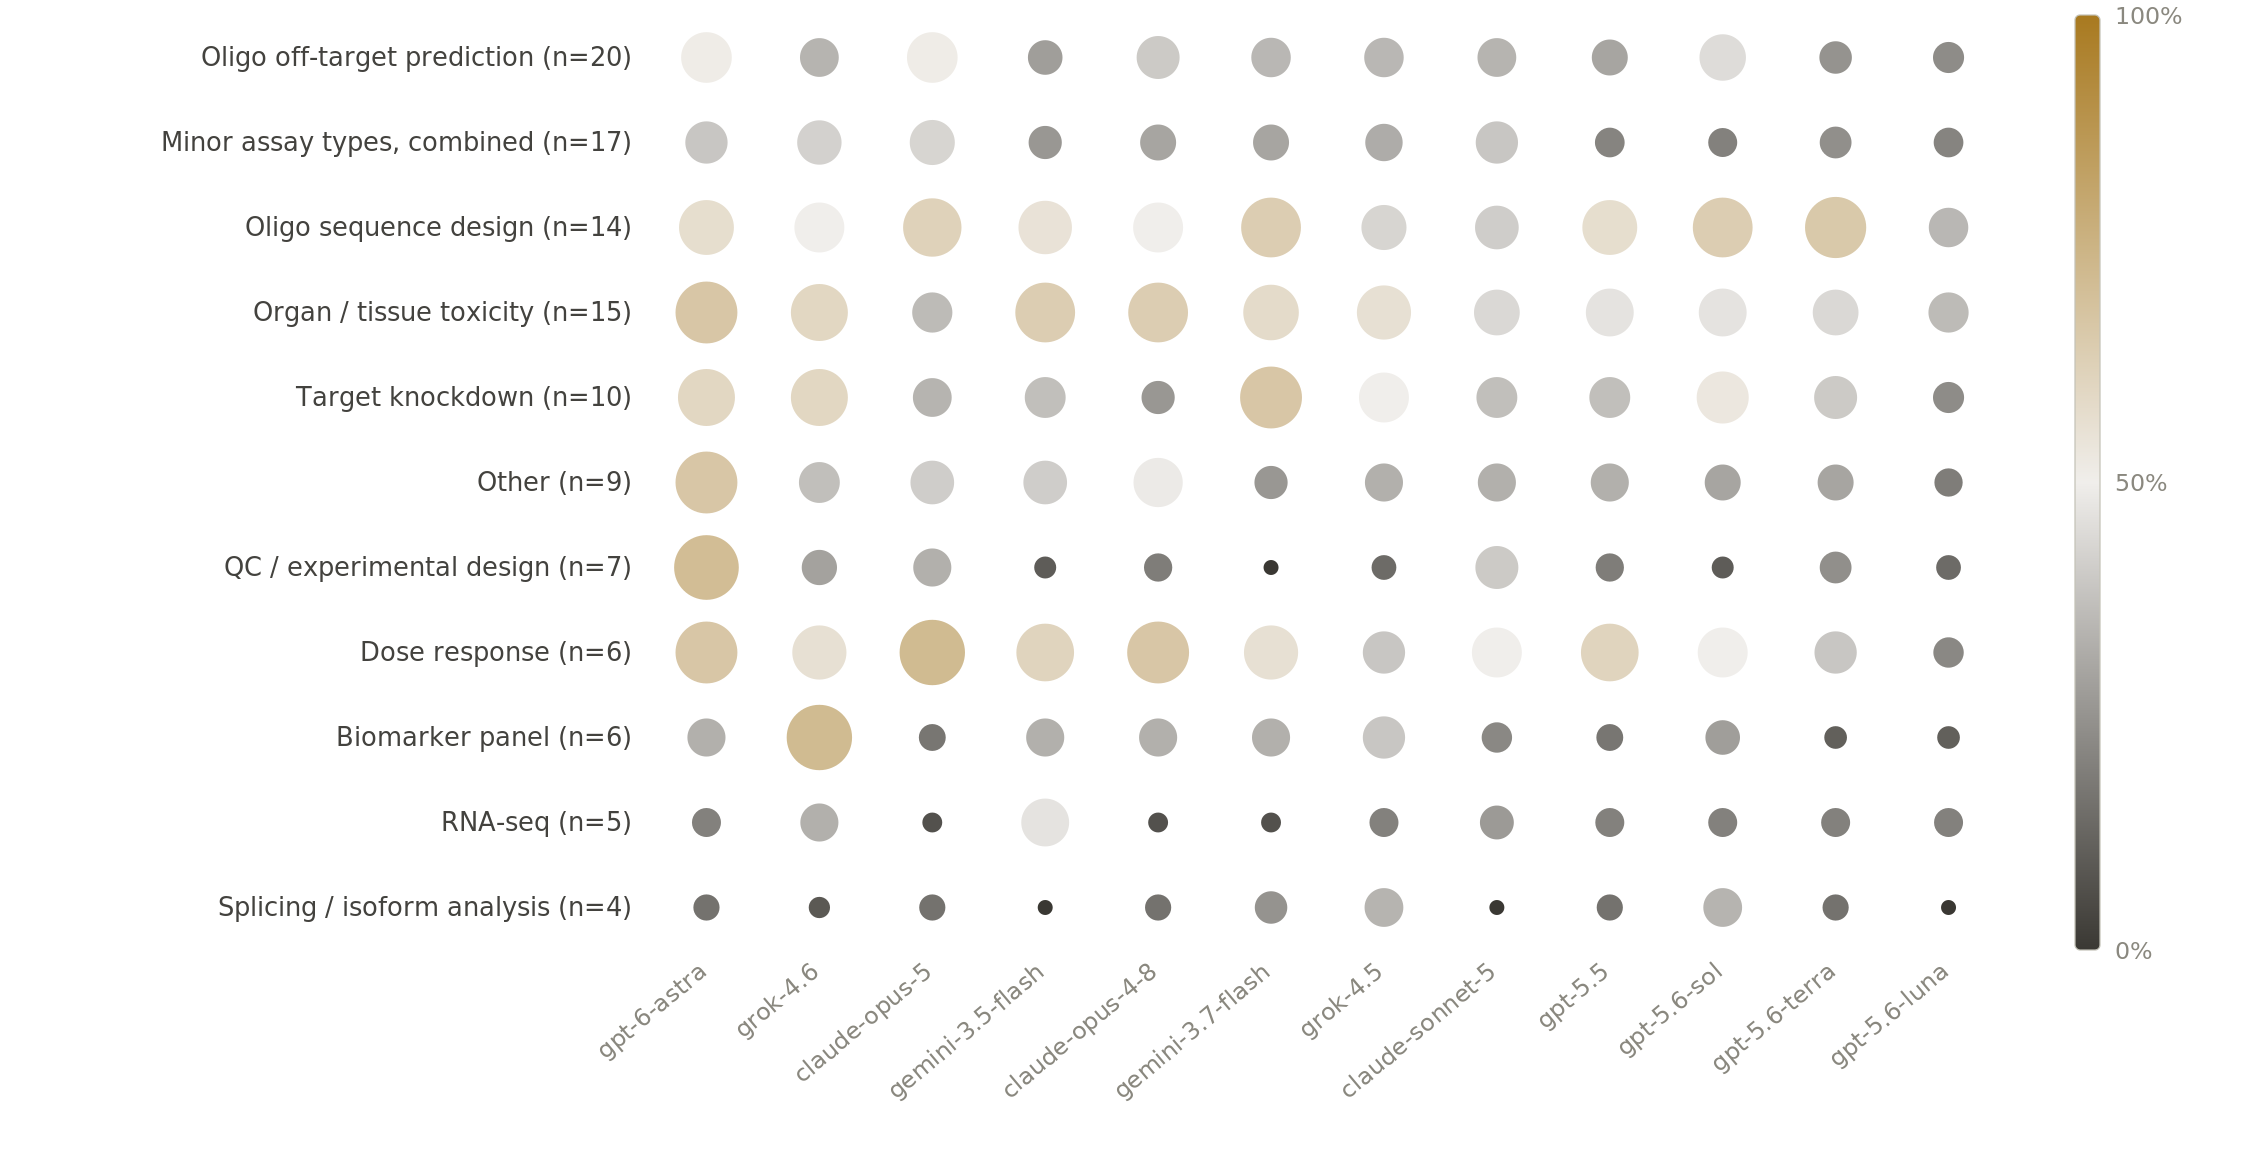
\includegraphics[width=\linewidth]{figures/chart-full-assay.png}
\end{subfigure}
\vspace{0.6em}
\caption{\textit{Pass rate by assay type.} \quad Pass rate by assay type (a derived, keyword-based grouping; top 10 types shown, the rest pooled) and model.}
\label{fig:fig8}
\end{figure}
\textbf{Time horizon, grader complexity, and failure modes all leave a mark on pass rate.} Time horizon distinguishes short-form evaluations, which ask for a single decision from one experimental snapshot, from long-form evaluations, which require tracking a decision across a sequence of timepoints or experiments (Figure 9A); long-form evaluations (n=14) show a lower overall pass rate than short-form (n=99), but this difference is not statistically significant (p=0.72; permutation test). Grader complexity shows no clean monotonic relationship to pass rate across the full campaign (Figure 9B) with standard errors overlap across most adjacent complexity levels, and even the largest step, from 35.3\% at complexity 4 to 57.6\% at complexity 5, reads as a modest bump against that full range rather than a real trend. The per-evaluation failure-mode tag (Figure 2E) predicts real difficulty directly, ahead of the full model-trajectory failure review: mean pass rate for evaluations carrying each individual tag ranges from 14\% to 37\% (Figure 9C).

\begin{figure}[p]
\centering
  \begin{subfigure}[t]{0.47\textwidth}
  \centering
  \caption{Time horizon}
  \label{fig:chart-timehorizon}
  \vspace{2pt}
  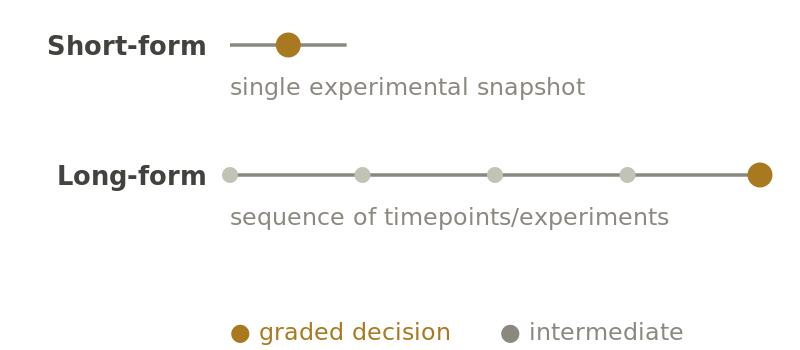
\includegraphics[width=\linewidth]{figures/chart-timehorizon.png}
  
\vspace{4pt}
\begin{center}
\small
\begin{tabular}{@{}lcc@{}}
\toprule
 & \textbf{Short-form} & \textbf{Long-form} \\
 & n=99 & n=14 \\
\midrule
Pass rate & 38.7\% & 36.7\% \\
 & 2,408/6,221 & 322/877 \\
\bottomrule
\end{tabular}
\end{center}

\end{subfigure}\hfill
  \begin{subfigure}[t]{0.47\textwidth}
  \centering
  \caption{Grader complexity vs. pass rate}
  \label{fig:chart-complexity}
  \vspace{2pt}
  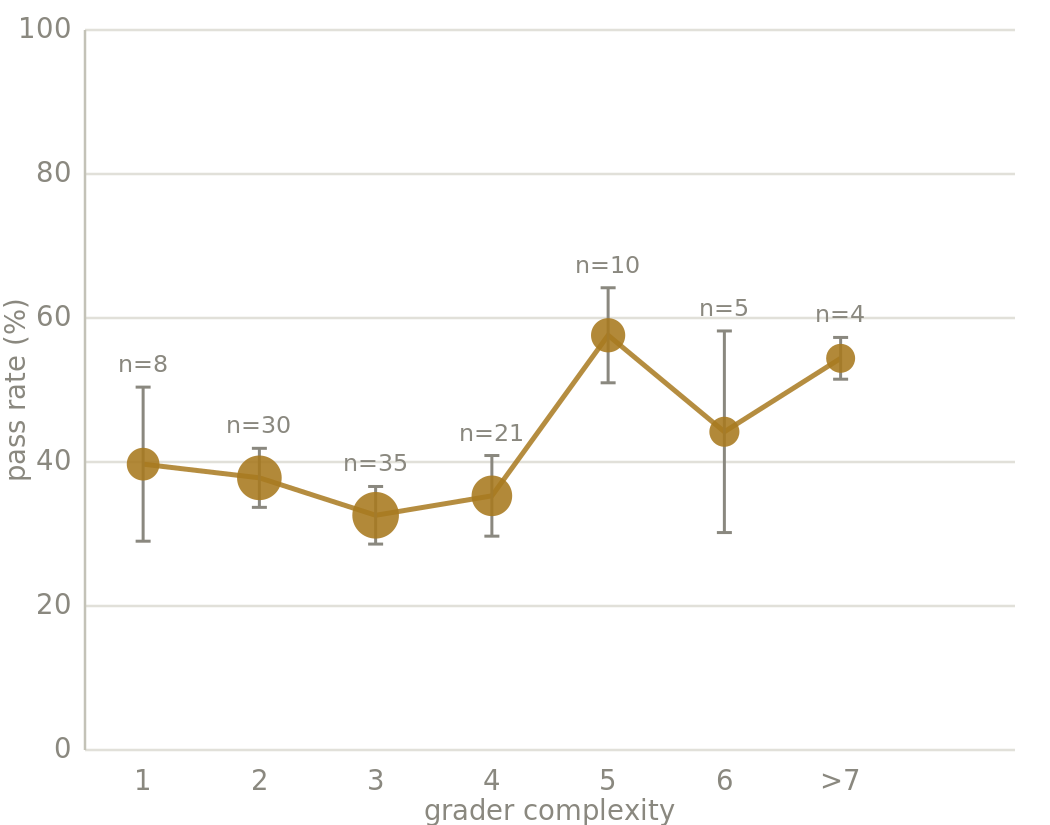
\includegraphics[width=\linewidth]{figures/chart-complexity.png}
\end{subfigure}
\vspace{0.6em}
  \hfill\begin{subfigure}[t]{0.6\textwidth}
  \centering
  \caption{Failure-mode tag vs. pass rate}
  \label{fig:chart-failuremode-pr}
  \vspace{2pt}
  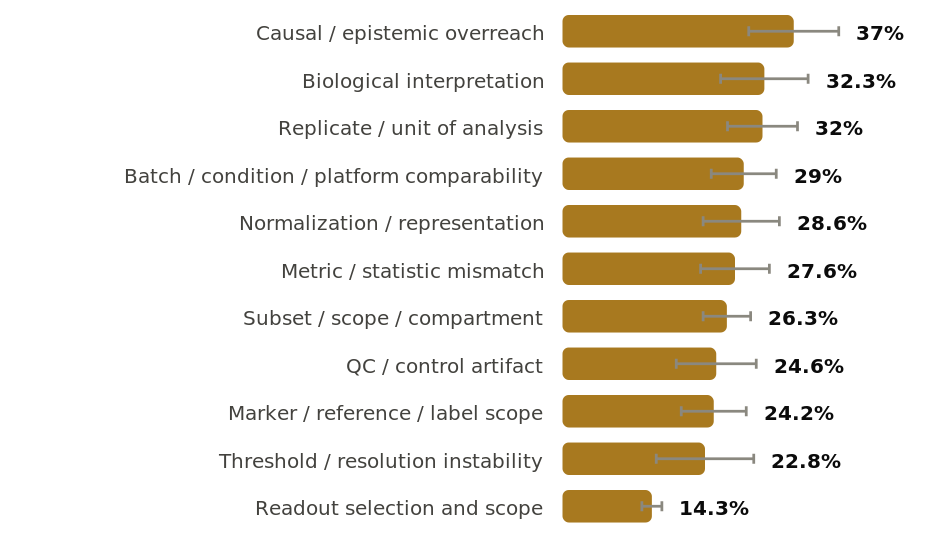
\includegraphics[width=\linewidth]{figures/chart-failuremode-pr.png}
\end{subfigure}\hfill\mbox{}
\vspace{0.6em}
\caption{\textit{Time horizon, grader complexity, and failure-mode tags.} \quad \textbf{A,} Pass rate by time-horizon tag: short-form (single-timepoint) versus long-form (multi-timepoint) evaluations, pooled across all 21 configurations. \textbf{B,} Pass rate versus grader complexity pooled across all 21 configurations; error bars are $\pm$1 standard error of the mean over per-evaluation pass rates within each complexity level. \textbf{C,} Mean pass rate for evaluations carrying each per-evaluation failure-mode tag, sorted descending; error bars are $\pm$1 standard error of the mean over per-evaluation pass rates within each tag. Categories are not mutually exclusive: an evaluation can carry more than one tag, so each bar is an independent mean over its own, overlapping subset of evaluations rather than a share of a fixed total; bars are not expected to sum to 100\%.}
\label{fig:fig9}
\end{figure}
\textbf{More computation does not consistently improve accuracy.} Cost and token accounting (Figure 10A--B) show more spend does not reliably buy accuracy: GPT-6 Astra on Pi reaches 53.4\% at \$0.20/run, cheaper than several configurations passing 15--20 points less. The dashed line traces the true cost/pass-rate Pareto frontier, the configurations no other configuration beats on both cost and pass rate simultaneously, not a per-family comparison: on cost, the frontier is defined entirely by two configurations, gpt-5.6-luna and GPT-6 Astra, each on both harnesses (the same four points Figure 10C lists explicitly); every Claude, Gemini, and Grok configuration is dominated by at least one of them, cheaper or more accurate or both. The token-based frontier (Figure 10B) is narrower still: GPT-6 Astra's two harnesses are the only two configurations on it, from 0.135M tokens/run (53.4\%) to 0.238M tokens/run (55.5\%).

\begin{figure}[p]
\centering
  \begin{subfigure}[t]{0.47\textwidth}
  \centering
  \caption{Pass rate vs.\ cost}
  \label{fig:chart-full-cost}
  \vspace{2pt}
  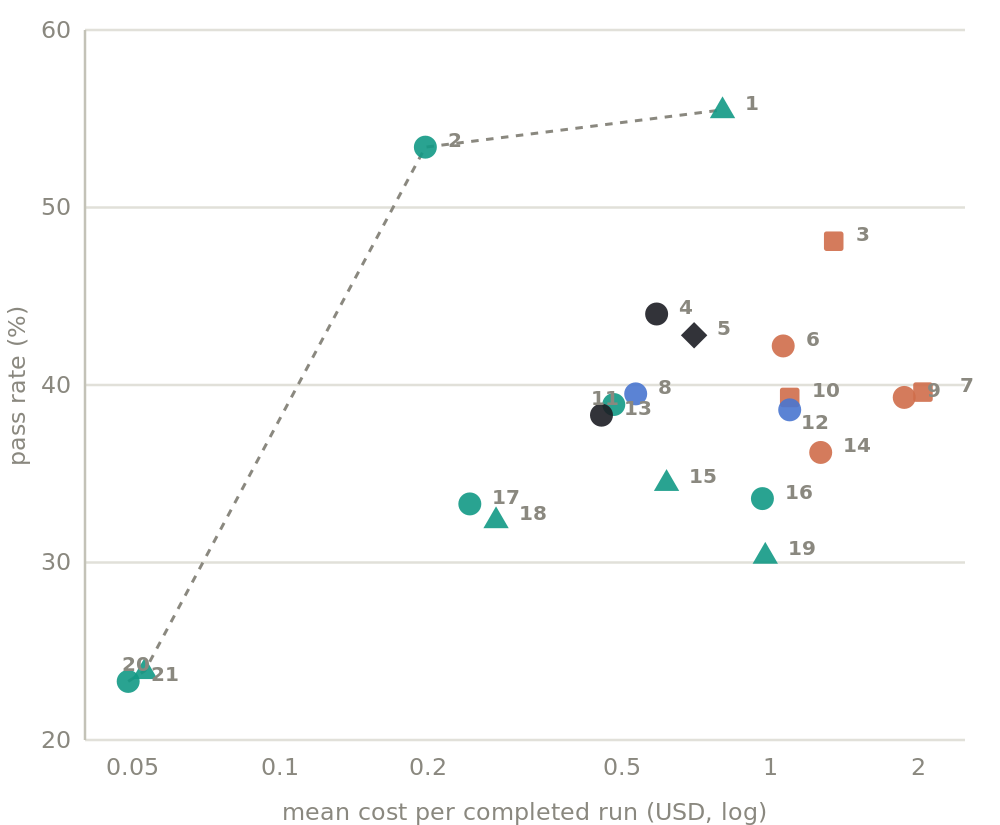
\includegraphics[width=\linewidth]{figures/chart-full-cost.png}
\end{subfigure}\hfill
  \begin{subfigure}[t]{0.47\textwidth}
  \centering
  \caption{Pass rate vs.\ token usage}
  \label{fig:chart-full-tokens}
  \vspace{2pt}
  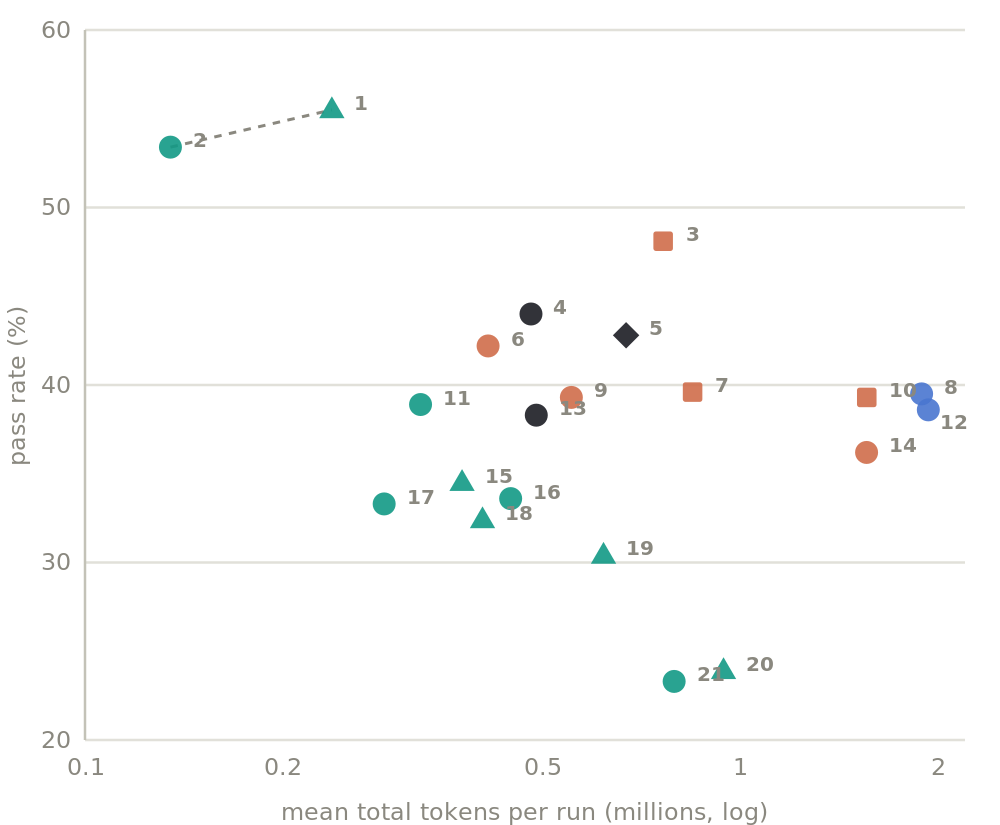
\includegraphics[width=\linewidth]{figures/chart-full-tokens.png}
\end{subfigure}
\vspace{0.6em}
\footnotesize\noindent\textbf{Model family:} \swatch{claudecol} Claude \quad \swatch{gptcol} GPT \quad \swatch{geminicol} Gemini \quad \swatch{grokcol} Grok \\
\textbf{Harness marker:} $\bullet$ Pi \quad $\blacksquare$ Claude Code \quad $\blacktriangle$ OpenAI Codex \quad $\blacklozenge$ Grok Build\normalsize\medskip

\noindent\textbf{Configuration ranking (by pass rate)}\smallskip

\begin{multicols}{3}\footnotesize
\begin{enumerate}[itemsep=0pt,parsep=0pt,topsep=0pt,leftmargin=1.6em]
\item gpt-6-astra / OpenAI Codex
\item gpt-6-astra / Pi
\item claude-opus-5 / Claude Code
\item grok-4.6 / Pi
\item grok-4.6 / Grok Build
\item claude-opus-5 / Pi
\item claude-opus-4-8 / Claude Code
\item gemini-3.7-flash / Pi
\item claude-opus-4-8 / Pi
\item claude-sonnet-5 / Claude Code
\item gpt-5.6-sol / Pi
\item gemini-3.5-flash / Pi
\item grok-4.5 / Pi
\item claude-sonnet-5 / Pi
\item gpt-5.6-sol / OpenAI Codex
\item gpt-5.5 / Pi
\item gpt-5.6-terra / Pi
\item gpt-5.6-terra / OpenAI Codex
\item gpt-5.5 / OpenAI Codex
\item gpt-5.6-luna / OpenAI Codex
\item gpt-5.6-luna / Pi
\end{enumerate}
\end{multicols}
\smallskip
\begin{center}\textbf{Cost/pass-rate frontier}\end{center}\smallskip
\begin{center}
\small
\begin{tabular}{lrrr}
\toprule
Config & \$/run & Pass \% & \$/correct \\
\midrule
gpt-5.6-luna (Pi) & \$0.049 & 23.3\% & \$0.210
\\
gpt-5.6-luna (OpenAI Codex) & \$0.053 & 23.9\% & \$0.222
\\
gpt-6-astra (Pi) & \$0.198 & 53.4\% & \$0.371
\\
gpt-6-astra (OpenAI Codex) & \$0.800 & 55.5\% & \$1.441
\\
\bottomrule
\end{tabular}
\end{center}

\caption{\textit{Cost and token accounting.} \quad \textbf{A,} Pass rate versus mean cost per completed run (log-scale axis, y-axis truncated to 20--60\%); color marks model family, marker shape marks execution harness, the small number beside each point gives its rank by pass rate (1 = highest, matching the Configuration list at right), and the dashed line traces the cost/pass-rate Pareto frontier (the non-dominated configurations from Figure 10C). \textbf{B,} Pass rate versus mean token usage per completed run (log-scale axis, same y-axis and rank numbering as A); dashed line traces the analogous token/pass-rate Pareto frontier. \textbf{C,} The cost/pass-rate non-dominated configurations across the full campaign (independently computed as the true Pareto frontier over all 21 configurations, not the same as the per-family line in A--B), listed explicitly with cost per correct answer (cost per run divided by pass rate).}
\label{fig:fig10}
\end{figure}\section{Discussion}
\textbf{Frontier agents are not yet reliable oligonucleotide-discovery decision-makers.} Across the full campaign, no model--harness configuration exceeded 56\% of endpoint attempts; the strongest, GPT-6 Astra on OpenAI Codex, passed 55.5\% (95\% CI 47.2--63.7), and pooled across all 21 configurations agents passed just 38.5\% of valid grading runs (Figure 3A). Repeatability compounds the gap: even the strongest configurations fail all three attempts on roughly a third of evaluations (Figure 3B), so a single passing run is a weak signal of genuine competence on a given decision.

\textbf{Model specialization, not a uniform skill gap.} The per-evaluation failure-mode taxonomy is dominated by subset/scope/compartment errors  rather than by raw computational mistakes (Figure 2E), the same pattern reported for TxBench-Antibody and TxBench-PP. Rankings are not uniform across evaluations either: reducing every evaluation to a per-model pass/fail verdict and comparing all 66 pairs across the 12 models shows real structure rather than a single competence ordering, though not a clean per-family split: the gpt-5.x sub-family and grok-4.5/4.6 cluster tightly, Claude Sonnet 5 pairs most closely with Gemini 3.5 Flash rather than its own family, and GPT-6 Astra, the strongest configuration overall, sits apart from every other model at the greatest distance (Figure 5; Figure 6A). The failure-mode and similarity results together suggest that improving pooled pass rate and improving scope/comparator judgment are the most consequential.

\textbf{Relationship to prior work.} TxBench-Oligonucleotide Discovery extends a decision-centered benchmarking approach shared with TxBench-PP, TxBench-Antibody, and VariantBench. Across all three benchmarks, the strongest model--harness configurations passed roughly 40--60\% of endpoint attempts on realistic, decision-centered biology tasks, and the large majority of failures were attributed to scientific-judgment errors (scope, comparator, and estimand selection; cross-context portability; and evidentiary calibration) rather than to raw computational execution. TxBench-Oligonucleotide Discovery's failure-mode design taxonomy is consistent with this pattern. TxBench-Antibody additionally reported that model rankings reversed across competencies, decision types, and evidence sources; the agent-to-agent similarity results here (Figures 5--6) extend that finding. Importantly, although the benchmark currently does not saturate all task possibilities, it provides a representative sample of problems to measure agent performance against each other. 


\textbf{Conclusion.} TxBench-Oligonucleotide Discovery shows that frontier AI agents can recover a subset of decisions an ASO/siRNA discovery program depends on, but are not yet reliable enough to substitute for expert judgment: the strongest configuration, GPT-6 Astra on OpenAI Codex, passes just over half of endpoint attempts, and pooled across the full campaign agents pass just under two-fifths of valid grading runs. Failures concentrate in scope, comparator, and baseline selection rather than in raw computation, echoing the same failure pattern reported for TxBench-PP and TxBench-Antibody, and model performance is structured by pipeline stage and decision type rather than by a single uniform capability gap: the strongest configuration overall is not the strongest configuration for every kind of decision. A single leaderboard number is therefore the wrong basis for deciding which model to trust with which class of oligonucleotide discovery task.

\section{Methods}
Benchmark composition and data. TxBench-Oligonucleotide Discovery comprises 113 evaluations derived from 21 ASO/siRNA discovery programs. Each evaluation includes an agent-facing task, a deterministic grader (Figure 2D), and benchmark metadata recording its taxonomy section, internal task type, time-horizon classification, and (where populated) a failure-mode tag.

Task format and grading. All evaluations use deterministic grading over a structured final answer, built from typed leaf checks composed under all-must-pass conjunctions where an evaluation requires more than one check.

Models were run without internet access in an isolated sandbox with a set of scientific analysis tools installed, at their maximum available reasoning-effort. Agents were only able to access files that were provided in the task format.   

Outcome classification and aggregation. Per-evaluation pass rate is computed as correct results over valid grading runs; per-configuration pass rate (Figure 3A) is the mean of those per-evaluation rates, with 95\% Student-t confidence intervals over the per-evaluation means. Time-horizon (Figure 9A) and grader-complexity (Figure 9B) breakdowns pool correct and valid counts across all 21 model--harness configurations, grouping evaluations by the number of leaf checks composing each evaluation's grader and by its metadata.time\_horizon tag, respectively.

Execution reliability and cost outliers. Refusals and execution failures concentrate in the same two checkpoints and are largely the same event. Trajectory review traces them to Anthropic's API-level content-safety classifier declining mid-task (flagged internally as a `bio' refusal), not a sandbox, tooling, or grading defect. Within the approved 113-evaluation set, only claude-opus-4-8 and claude-sonnet-5 refuse---on three evaluations; claude-opus-5 never refuses on the same prompts and data. A fourth evaluation shows one isolated refusal that doesn't trigger a full exclusion. For these two checkpoints, every platform-level execution failure is also an API-level content refusal---one problem counted twice, not two (the sole exception: one unrelated, non-refusal platform failure for a third configuration, which doesn't affect its denominator). Because these failures track model version rather than task content, affected evaluations were dropped from the denominator rather than scored wrong, giving claude-opus-4-8 (n=111 on one harness, n=112 on the other) and claude-sonnet-5 (n=112 on both) slightly smaller samples than the nominal 113 (Figure 3A; Figure 4). The same two checkpoints also account for every cost outlier in the campaign: of eleven runs costing more than 8$\times$ their evaluation's median (up to \$25.82 against a \$2.46 median), seven are claude-opus-4-8 (six of which still failed, consistent with tool-loop or retry thrashing) and four are claude-sonnet-5---all on a single evaluation, all likewise incorrect.
\section*{References}
\begin{enumerate}[leftmargin=2em,itemsep=3pt]
\item Ramasamy, R., Le, H., Brougher, J., Urrutia, A., Banerjee, A., Poust, S. \& Workman, K. TxBench -- Antibody Discovery: Benchmarking AI Agents on Experimentally Grounded Decisions in Therapeutic Antibody Discovery. LatchBio.
\item Le, H., Ramasamy, R., Urrutia, A., Yazdani, M., Proctor, T. \& Workman, K. TxBench-PP: Analyzing AI Agent Performance on Small-Molecule Preclinical Pharmacology. \textit{arXiv:submit/7725456 [cs.AI]}, 17 June 2026.
\item Bhowmick, A., Rahmatpour, N., Sharma, S., Xu, Q., Gupta, A., Lagwankar, A., Banerjee, A. \& Zou, C. VariantBench: An Agentic Benchmark for Genetic Variant Discovery and Interpretation. LatchBio.
\item Hill, B., Jaques, M.R., Nair, R.R., Whiffin, N., Wood, M.J.A., Sanders, S.J., Oliver, P.L., Hill, A.C. \& Rinaldi, C. Accurately modeling RNase H-mediated antisense oligonucleotide efficacy. \textit{Molecular Therapy Nucleic Acids} 37(3):103004, 2026.
\item Sundar, A., Wei, Z. \& Griesmer, S. Benchmarking Large Language Models for Predicting Therapeutic Antisense Oligonucleotide Efficacy. \textit{bioRxiv} 2026.02.17.706455, 2026.
\item Andreone, B.J. et al. Durable suppression of seizures in a preclinical model of KCNT1 genetic epilepsy with divalent small interfering RNA. \textit{Epilepsia} 66(5):1677--1690, 2025.
\item Bäckström, E., Bonetti, A., Johnsson, P., Öhlin, S., Dahlén, A., Andersson, P., Andersson, S. \& Gennemark, P. Tissue pharmacokinetics of antisense oligonucleotides. \textit{Molecular Therapy Nucleic Acids} 35(1):102133, 2024.
\item Burdick, A.D. et al. Sequence motifs associated with hepatotoxicity of locked nucleic acid-modified antisense oligonucleotides. \textit{Nucleic Acids Research} 42(8):4882--4891, 2014.
\item Chen, X., Birey, F., Li, M.-Y., Revah, O., Levy, R., Thete, M.V., Reis, N., Kaganovsky, K., Onesto, M., Sakai, N., Hudacova, Z., Hao, J., Meng, X., Nishino, S., Huguenard, J. \& Pașca, S.P. Antisense oligonucleotide therapeutic approach for Timothy syndrome. \textit{Nature} 628(8009):818--825, 2024.
\item Didiot, M.C. et al. Nuclear localization of huntingtin mRNA is specific to cells of neuronal origin. \textit{Cell Reports} 24(10):2553--2560, 2018.
\item El Boujnouni, N., van der Bent, M.L., Willemse, M., 't Hoen, P.A.C., Brock, R. \& Wansink, D.G. Block or degrade? Balancing on- and off-target effects of antisense strategies against transcripts with expanded triplet repeats in DM1. \textit{Molecular Therapy Nucleic Acids} 32:622--636, 2023.
\item Golinski, S.R., Soriano, K., Briegel, A.C. et al. RNA targeting therapy for a prenatally enriched potassium channel associated with severe childhood epilepsy and premature death. \textit{Nature Communications} 17:5864, 2026.
\item Guo, S., Booten, S.L., Aghajan, M. et al. Antisense oligonucleotide treatment ameliorates alpha-1 antitrypsin-related liver disease in mice. \textit{Journal of Clinical Investigation} 124(1):251--261, 2014.
\item Hagedorn, P.H., Pontoppidan, M., Bisgaard, T.S. et al. Identifying and avoiding off-target effects of RNase H-dependent antisense oligonucleotides in mice. \textit{Nucleic Acids Research} 46(11):5366--5380, 2018.
\item Holgersen, E.M., Gandhi, S., Zhou, Y. et al. Transcriptome-wide off-target effects of steric-blocking oligonucleotides. \textit{Nucleic Acid Therapeutics} 31(6):392--403, 2021.
\item Janas, M.M., Jiang, Y., Schlegel, M.K., Waldron, S., Kuchimanchi, S. \& Barros, S.A. Impact of oligonucleotide structure, chemistry, and delivery method on in vitro cytotoxicity. \textit{Nucleic Acid Therapeutics} 27(1):11--22, 2017.
\item Klim, J.R., Williams, L.A., Limone, F. et al. ALS-implicated protein TDP-43 sustains levels of STMN2, a mediator of motor neuron growth and repair. \textit{Nature Neuroscience} 22(2):167--179, 2019.
\item Kuijper, E.C., van der Graaf, L., Pepers, B.A. et al. Determining off-target effects of splice-switching antisense oligonucleotides using short read RNAseq in neuronally differentiated human induced pluripotent stem cells. \textit{Human Molecular Genetics} 34(22):1912--1925, 2025.
\item Lee, H.-S., Seok, H., Lee, D.H., Ham, J., Lee, W., Youm, E.M., Yoo, J.S., Lee, Y.-S., Jang, E.-S. \& Chi, S.W. Abasic pivot substitution harnesses target specificity of RNA interference. \textit{Nature Communications} 6:10154, 2015.
\item McCampbell, A., Cole, T., Wegener, A.J. et al. Antisense oligonucleotides extend survival and reverse decrement in muscle response in ALS models. \textit{Journal of Clinical Investigation} 128(8):3558--3567, 2018.
\item Shen, W., De Hoyos, C.L., Sun, H., Vickers, T.A., Liang, X.H. \& Crooke, S.T. Acute hepatotoxicity of 2$'$ fluoro-modified 5--10--5 gapmer phosphorothioate oligonucleotides in mice correlates with intracellular protein binding and the loss of DBHS proteins. \textit{Nucleic Acids Research} 46(5):2204--2217, 2018.
\item Vickers, T.A., Rahdar, M., Prakash, T.P. \& Crooke, S.T. Kinetic and subcellular analysis of PS-ASO/protein interactions with P54nrb and RNase H1. \textit{Nucleic Acids Research} 47(20):10865--10880, 2019.
\item Wheeler, T.M., Leger, A.J., Pandey, S.K. et al. Targeting nuclear RNA for in vivo correction of myotonic dystrophy. \textit{Nature} 488(7409):111--115, 2012.
\item Popper, K. The Logic of Scientific Discovery. Basic Books, 1959.
\item Duhem, P. The Aim and Structure of Physical Theory. Princeton University Press, 1954.
\item Quine, W.V.O. Two Dogmas of Empiricism. \textit{The Philosophical Review} 60(1):20--43, 1951.
\end{enumerate}
\end{document}
